%Made By Thomas Debelle
%Ajouté des Packages si nécessaires
\documentclass{report}
\usepackage[a4paper, total={7.5in, 10.5in}]{geometry}
\usepackage[utf8]{inputenc}
\usepackage[english]{babel}
\usepackage{graphicx}
\usepackage{graphics}
\usepackage[T1]{fontenc}
\usepackage{amsmath}
\usepackage{hyperref}
\usepackage{amssymb}
\usepackage{listings}
\usepackage{xcolor}
\usepackage{array}
\usepackage{float}
\usepackage{amsfonts}
\usepackage{fancyhdr}
\usepackage{titlesec}
\usepackage{pdfpages}
\usepackage{xparse}
\usepackage{wrapfig}
\usepackage{booktabs}
\usepackage{colortbl}

\usepackage{listings}
\usepackage[dvipsnames]{xcolor}

\definecolor{codegreen}{rgb}{0,0.6,0}
\definecolor{codegray}{rgb}{0.5,0.5,0.5}
\definecolor{codepurple}{rgb}{0.58,0,0.82}
\definecolor{backcolour}{rgb}{0.95,0.95,0.92}

\lstdefinestyle{mystyle}{
    backgroundcolor=\color{backcolour},   
    commentstyle=\color{codegreen},
    keywordstyle=\color{magenta},
    numberstyle=\tiny\color{codegray},
    stringstyle=\color{codepurple},
    basicstyle=\ttfamily\footnotesize,
    breakatwhitespace=false,         
    breaklines=true,                 
    captionpos=b,                    
    keepspaces=true,                 
    numbers=left,                    
    numbersep=5pt,                  
    showspaces=false,                
    showstringspaces=false,
    showtabs=false,                  
    tabsize=2
}

\lstset{style=mystyle}

\hypersetup{
    colorlinks=true,
    linkcolor=black,
    filecolor=magenta,
    urlcolor=cyan,
    pdftitle={Overleaf Example},
    pdfpagemode=FullScreen,
    }
\begin{document}
% RISC-V Assembler syntax and style for latex lstlisting package
% 
% These are risc-v commands as per our university (University Augsburg, Germany) guidelines.
%
% Author: Anton Lydike
%
% This code is in the public domain and free of licensing

% language definition
\lstdefinelanguage[RISC-V]{Assembler}
{
  alsoletter={.}, % allow dots in keywords
  alsodigit={0x}, % hex numbers are numbers too!
  morekeywords=[1]{ % instructions
    lb, lh, lw, lbu, lhu,
    sb, sh, sw,
    sll, slli, srl, srli, sra, srai,
    add, addi, sub, lui, auipc,
    xor, xori, or, ori, and, andi,
    slt, slti, sltu, sltiu,
    beq, bne, blt, bge, bltu, bgeu,
    j, jr, jal, jalr, ret,
    scall, break, nop
  },
  morekeywords=[2]{ % sections of our code and other directives
    .align, .ascii, .asciiz, .byte, .data, .double, .extern,
    .float, .globl, .half, .kdata, .ktext, .set, .space, .text, .word
  },
  morekeywords=[3]{ % registers
    zero, ra, sp, gp, tp, s0, fp,
    t0, t1, t2, t3, t4, t5, t6,
    s1, s2, s3, s4, s5, s6, s7, s8, s9, s10, s11,
    a0, a1, a2, a3, a4, a5, a6, a7,
    ft0, ft1, ft2, ft3, ft4, ft5, ft6, ft7,
    fs0, fs1, fs2, fs3, fs4, fs5, fs6, fs7, fs8, fs9, fs10, fs11,
    fa0, fa1, fa2, fa3, fa4, fa5, fa6, fa7
  },
  morecomment=[l]{;},   % mark ; as line comment start
  morecomment=[l]{\#},  % as well as # (even though it is unconventional)
  morestring=[b]",      % mark " as string start/end
  morestring=[b]'       % also mark ' as string start/end
}

% usage example:

% define some basic colors
\definecolor{mauve}{rgb}{0.58,0,0.82}



%Si la mention "Juin 2023" est sur une autre page, changé le dernier VSPACE
\begin{titlepage}
    \begin{figure}
        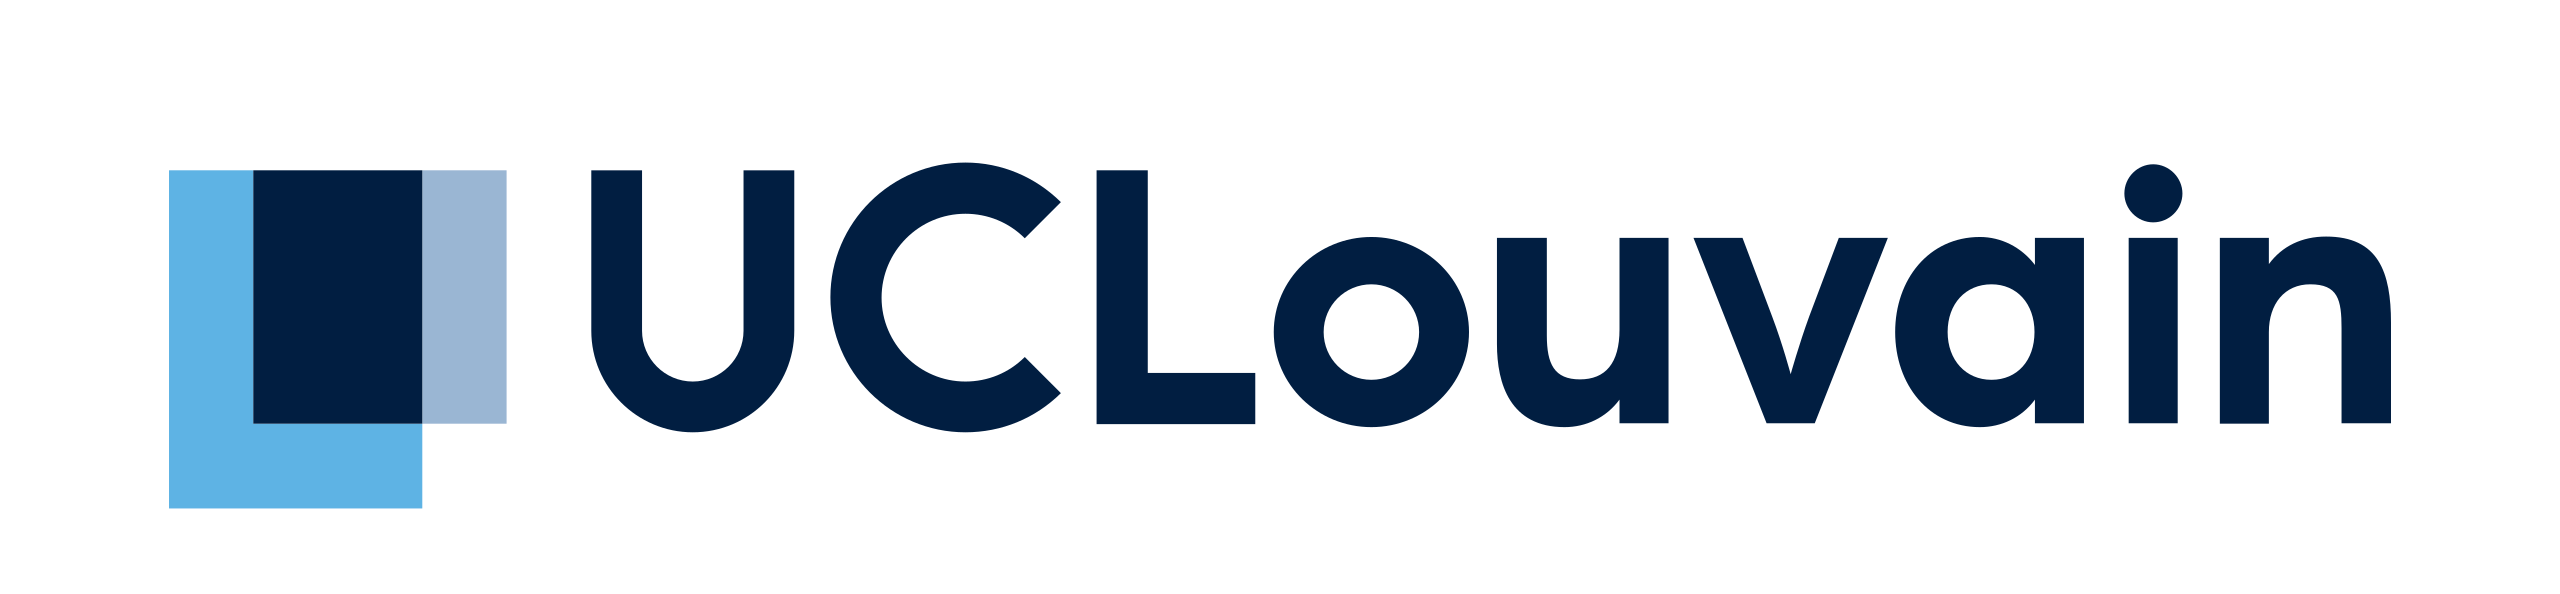
\includegraphics[height = 2cm]{UCL_Logo.png}
        \label{fig:my_label}
    \end{figure}

    \hspace*{100cm}
    \centering
    \vspace*{7cm}

    {\Huge \textbf{Summary Computer Architecture}}\\
    \vspace*{0.25cm}
    Compiled on \today\\
    \vspace*{0.25cm}
    \Large{Noms des Auteurs}\\

    \vspace*{9.5cm} %Le dernier VSPACE
    {\Large Juin 2023}
\end{titlepage}

%_____NE PAS MODIFIER______
\tableofcontents
\newpage

%_______Vous pouvez modifier en-dessous_____

\chapter{Recap of pipelined processor}

\section{ISA}

Stands for \textbf{I}nstruction \textbf{S}et \textbf{A}rchitecture : 
\begin{enumerate}
    \item CISC : Complex instruction set computer : VAX, X86
    \item RISC : Reduced instruction set computer : ARM, MIPS, SPARC, RISC-V
\end{enumerate}

When we talk about RISC-V we always use \textbf{32 bits instructions} and \textbf{xx bits data and address space}. Typical name is RVxxI : RV64I in this course. We also have multiples types in RISC-V of instructions :

\begin{enumerate}
    \item R : \textbf{Arithmetic} : we always need to specify the output register and the two input registers.
    \item I : \textbf{Immediate} : they are similar to R-type but now we can add some \textit{immediate} instead of an input register. \textbf{Important} the immediate is maximum 12 bits so we need to use some tricks to use 64 bits immediate.
    \item S : \textbf{Store} : used  to store data, needs to read and write from multiple registers (data, destination). \textit{Note:} to load we are using  the I-type since we just need the destination, address register and an immediate to offset.
    \item B : \textbf{Branch} : allows us to create some specific condition to maybe trigger some subroutine when combined with Jump instruction.
    \item J : \textbf{Jump} : used to jump to other part of the code. Jump and link allows us to jump further than using the Jump and link reg since this one uses the I-type instruction format.
    \item U :
\end{enumerate}

\begin{lstlisting}[language=C]
    // Typical R type
    add x1, x2, x3 // x1 = x2 + x3
\end{lstlisting}

In R-type, we use rs1, rs2 and rd as 5 bits describing the address register (super small memory !). The opcode serves as an indication of which type is used and the \textit{funct7} and \textit{funct3} are used as function codes augmenting the opcode.\\
Immediate can be maximum 12 bits as indicated in the RISC-V card. We don't use a funct7 anymore. Important to notice the \textit{regularity} of the bits in the different type, aligning them makes it easier and requires less multiplexer, ...\\
Load instuction are like this  : \verb|ld x1, 24(x2)| where we have the rd as x1 and x2 serves to indicate the address in the DM, the immediate indicates how much we need to jump (good for iterating) usually the immediate is a multiple of 8 since we are working with 64 bits memory word.\\
The store instruction is like \verb|sd x2, 24(x1)|. Important to notice that we don't have any rd register ! So that's the reason why we use another structure. Indeed to store we just need a register containing the value, the address and an immediate to jump in the memory. So indeed no need to have a result register \textit{rd}.\\
For branching it is important to notice how the various way to jump leads to various type having some limitations and perks. To gain some reach, we are not using the MSB of the immediate which is 1 and adds non useful granularity. \textbf{WHY THIS WEIRD SPLIT ?}. The jump and link is of type J which is perfect to quickly jump further than needed since we just have rd and no other rs and we can even remove the funct 7 and 3 since it is an unique type for this instructions.

\begin{lstlisting}[language=C]
// C
while(save[i] == k)
    i += 1;

// RISC-V code
Loop:
    add  x1, x3, x6
    ld   x2, 0(x1)
    bne  x2, x5, Exit
    addi x3, x3, 8
    jal  x0, Loop
Exit:
    ...
\end{lstlisting}

\begin{wrapfigure}{r}{0.28\textwidth}
  \begin{center}
        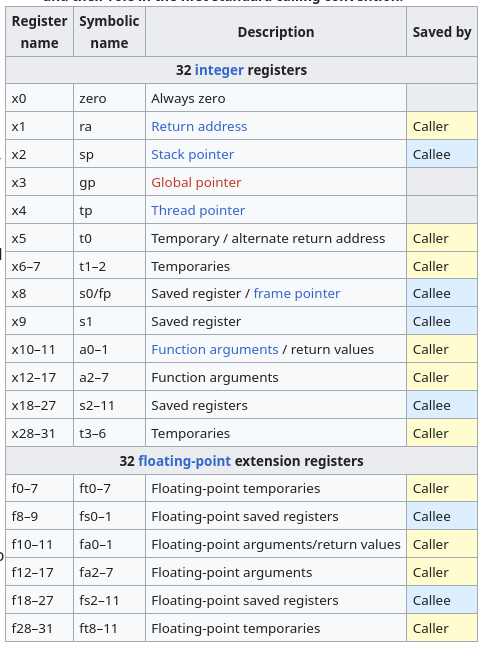
\includegraphics[width=0.9\linewidth]{caller_callee.png}
        \label{fig:caller-callee}
  \end{center}
\end{wrapfigure}

It is interesting to notice how the tag \textit{Exit} will be converted to a relative jump instead of an absolute to the line 12 for example.

\subsection{Return loops and nesting subroutine}



When we do a \verb|jal| we save in \verb|ra| the current program counter but after resuming and calling other functions, we have no guarantee that this register won't be changed !

We have some conventions in RISC-V regarding some registers and their use but also who "owns" it and is allowed to tweak its value. In other words, it creates some cohesion between developer and indicates what registers we may expect their value to be changed before and after a call.


\subsection{Pseudo-instruction}
\label{macro}

We will sometimes use \verb|li| which is a pseudo instruction which helps with loading large immediate values than are bigger than 12 bits :\\

\begin{lstlisting}[language=C]
    li   x5, 0xB34FE0A3

    // Becomes
    lui  x5, 0XB34FE
    addi x5, x5, 0X0A3
\end{lstlisting}

\begin{lstlisting}[language=C,caption=Other Pseudo instructions]
    nop                 addi x0, x0, 0              //No operation
    li rd, imm          //Myriad sequences          Load immediate
    mv rd, rs           addi rd, rs, 0              //Copy register
    beqz rs, offset     beq rs, x0, offset          //Branch if zero
    j offset            jal x0, offset              //Jump
    call offset         auipc x1, offset[31:12]     //Call far-away subroutine
                        jalr x1, x1, offset[11:0]
\end{lstlisting}




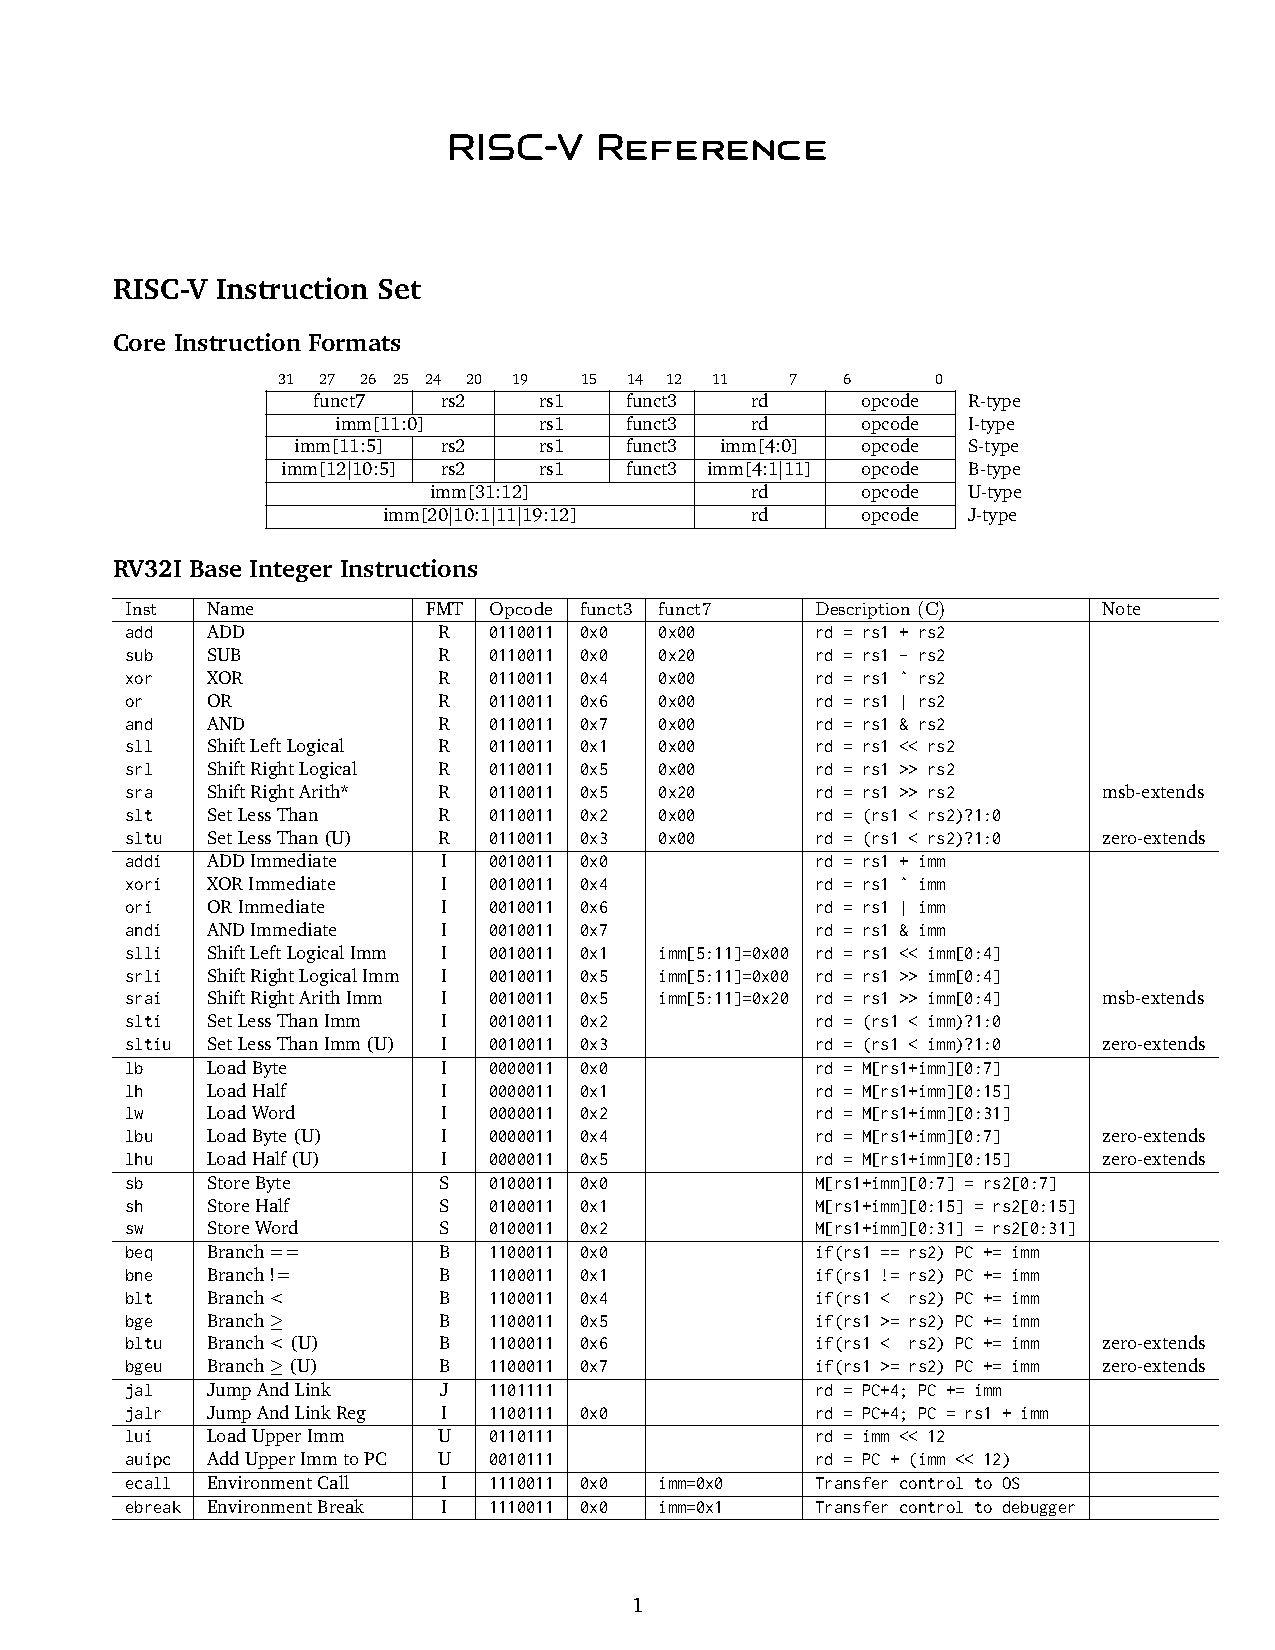
\includepdf[pages=1]{RISCV_CARD.pdf}

\section{Single cycle processor}
\label{scp}
\begin{figure}[H]
    \centering
    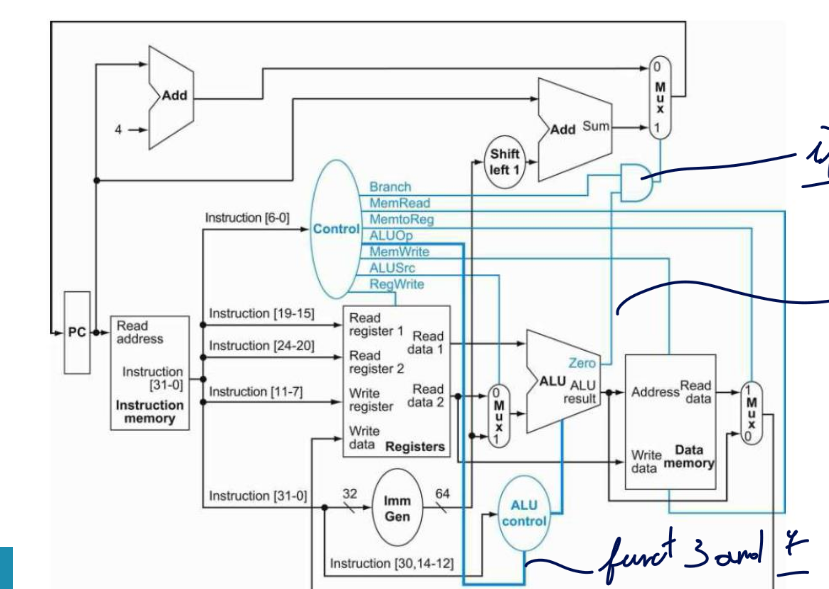
\includegraphics[width=0.65\linewidth]{single_cycle_proc.png}
    \caption{Single Cycle Processor}
    \label{fig:enter-label}
\end{figure}

We usually first \textbf{fetch} the instruction (so moving the program counter to see which line we need to run next). So updating the program counter in 32 bits instruction requires to move 4 bytes at each time hence the +4. It is important to notice that reading from memory is \textit{unclocked} while writing to memory is \textit{clocked}, this allows that the instruction read won't take an extra clock cycle and will propagate directly resulting in a more efficient CPU.\\
Then we \textbf{decode}, here we can see why aligning data and instruction matters, we need less multiplexer. We can read  up to 2 registers and write to one the data.\\
After this, we \textbf{execute} and we expect the control unit to properly set the signal for the ALU and other components to properly execute the various instructions. Important to notice that the data 1 and 2 going through the ALU are \textbf{64 bits} in RISC64I.

\section{Pipelined processor}

We can start back from the simple Single cycle processor (\ref{scp}) and simply at registers along the way. But watch out, this will increase latency but can improve throughput since we have a relaxed timing. Of course, we can't neglect the energy and power usage of such registers and other physical phenomena.\\

In the classic 5 stages pipelined processor we have : 

\begin{enumerate}
    \item \textbf{IF} : Instruction fetch from memory
    \item \textbf{ID} : Instruction decode \& register read
    \item \textbf{EX} : Execute operation (or add offset to address)
    \item \textbf{MEM} : Access memory operand
    \item \textbf{WB} : Write result back to register
\end{enumerate}

\begin{figure}[H]
    \centering
    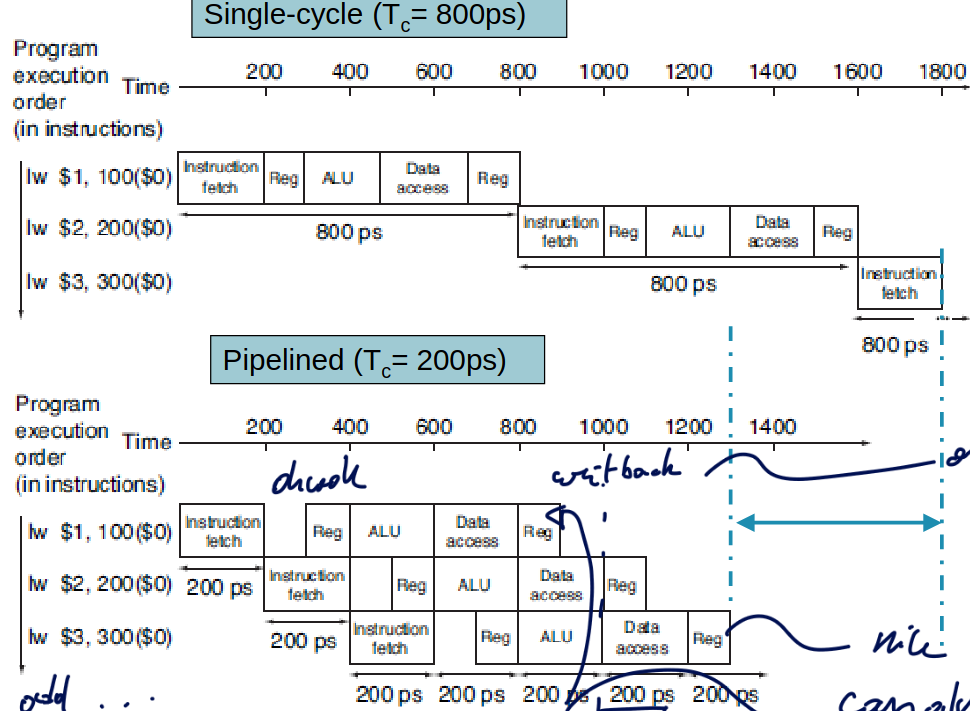
\includegraphics[width=0.75\linewidth]{5_stage_proc.png}
    \caption{5 stages pipelined processor}
    \label{fig:5-stage-label}
\end{figure}

Notice here that we write back on falling edge of the clock while we read on raising clock. This is done so the read of a future instruction can use fresh memory and do not need to wait for an extra clock cycle.\\

One of the most important metric is the CPU time : 

\begin{equation}
    CPU \quad time = \underbrace{\frac{Instructions}{Program}}_{Instruction \quad Count} \cdot \underbrace{\frac{Clock \quad Cycles}{Instruction}}_{CPI} \cdot \underbrace{\frac{Seconds}{Clock \quad Cycles}}_{Clock \quad Cycle \quad Time}
    \label{eq:fundamental_perf}
\end{equation}

Pipelining will improve the clock cycle time and will slightly worsen the CPI due to the fact we will have some data and control hazard.

\subsection{Data hazard}


\begin{wrapfigure}{r}{0.5\textwidth}
    \centering
    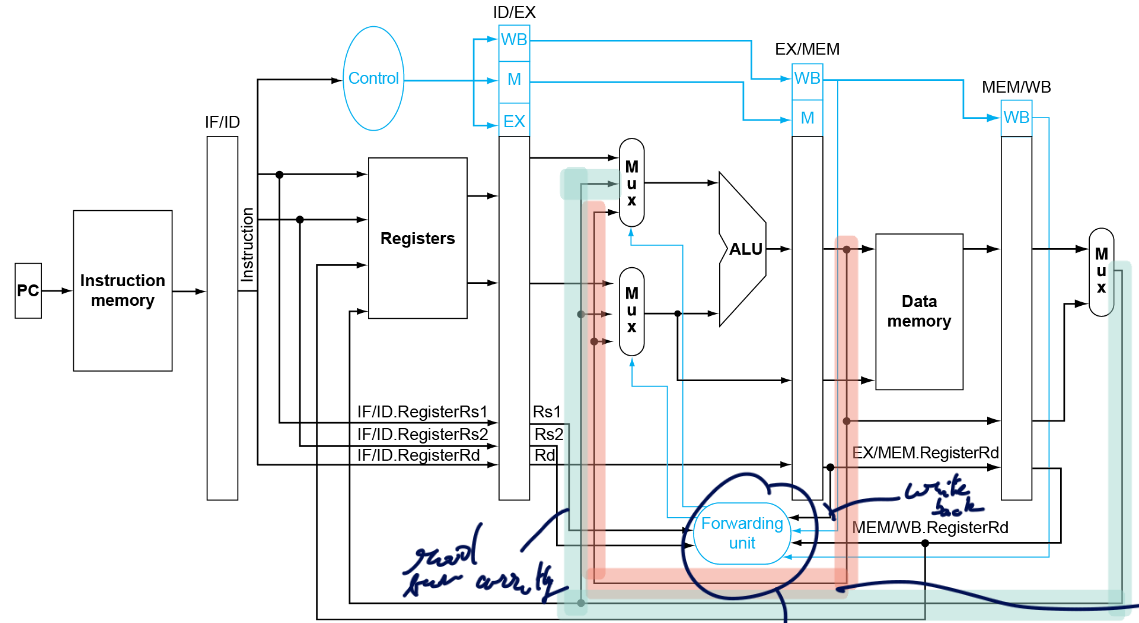
\includegraphics[width=0.95\linewidth]{data_hazard_bypass.png}
    \caption{Bypassing in the 5 stage CPU}
    \label{fig:hazard-control-label}
\end{wrapfigure}

One approach is a \textit{static} approach where the compiler can add some \textbf{NOP} to let the processor do meaningless operation while waiting to get the memory write back. Or the compiler can be a little smart and reshuffle some instruction if it sees that there is no data dependencies.\\

A better approach is a \textit{dynamic} or processor based approach where we are going to introduce \textbf{forwarding/bypassing}. We are going to create some wires that can go from the ALU to the input of the ALU in case this data is needed for the next clock cycle.\\

This forwarding unit block can be prorgrammed in verilog with :

\begin{lstlisting}[language=verilog, caption=data hazard]
if [EX/MEM.RegWrite and (EX/MEM.RegisterRd != x0) 
    and (EX/MEM.RegisterRd == ID/EX.RegisterRs1) ]
        ForwardA = 2 // The red wire

if [ MEM/WB.RegWrite and (MEM/WB.RegisterRd != x0)
    and (MEM/WB.RegisterRd = ID/EX.RegisterRs1) ]
    and not[ EX/MEM.RegWrite and (EX/MEM.RegisterRd != x0)
    and (EX/MEM.RegisterRd == ID/EX.RegisterRs1) ]
        ForwardA = 1 // The blue wire
\end{lstlisting}

The added \textit{not} in the second condition is there so we don't have a concurrent bypass of data. So we will always use the most recent version for bypassing (here the red wire from the ALU).\\

But sometimes we don't just want to access from the ALU but after a read ! For example in a load instruction the data after the memory access is of interest. In that case, we are forced to add a NOP and to stall the pipeline. To do this we will simply not change the program counter to fetch the instruction after the NOP bubble. We call this \textit{stalling the pipeline}.

\begin{lstlisting}[language=verilog, caption=load data hazard]
If (ID/EX.MemRead ==1   //load
    and ((ID/EX.RegisterRd == IF/ID.RegisterRs1) or
    (ID/EX.RegisterRd == IF/ID.RegisterRs2))
        stall pipeline      // NOP
\end{lstlisting}

\subsection{Control hazard}

Again, we can have a \textit{static} approach where the compiler will add some NOP or do some loop unrolling to avoid too many branches.\\

But a better approach is \textit{dynamic} where the processor controls the branches and will predict and flush if wrong. To flush, it is important the the wrong instructions didn't access the register write back stage or that it didn't change a value in RAM or the drive. After flushing, we can fetch the correct instruction.

\begin{figure}[H]
    \centering
    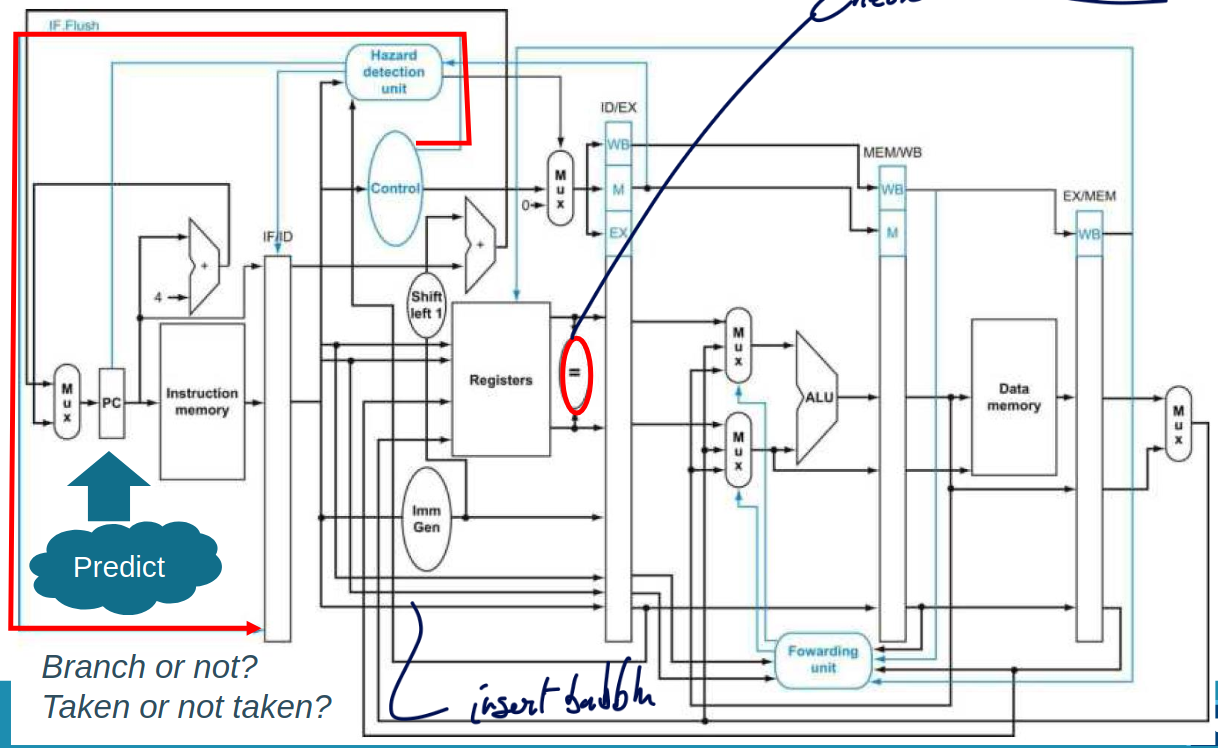
\includegraphics[width=0.75\linewidth]{flushing_pipeline.png}
    \caption{Flushing pipeline}
    \label{fig:flush-label}
\end{figure}

With this approach, we will only lose 1 clock cycle after the registers read which will feedback any issue. We will insert those NOP operation if we see that the branch prediction wasn't correct. We have some simple branch prediction schemes : 

\begin{enumerate}
    \item \underline{Simple prediction :} branch not taken $30-40 \%$ accuracy.
    \item \underline{Static prediction :} if branch to forward PC do not take if branch to backward PC do take. $60-70 \%$ accuracy. Better accuracy because it is based on usual programming where we loop a lot and sometimes throw exception (see chap. \ref{part-3}).
\end{enumerate}

\section{Architecture variants}

RV64I is simply an ISA so we are free to implement it as we would like. Some implementation can reduce or not the amount of bubble it needs to insert for compute-use, load-use and branch instruction. This always depend on the specific implementation of the CPU.


\section{Instruction extensions}

We can add some variants to spice up our ISA and make it more efficient or better at specific task.

\begin{figure}[H]
    \centering
    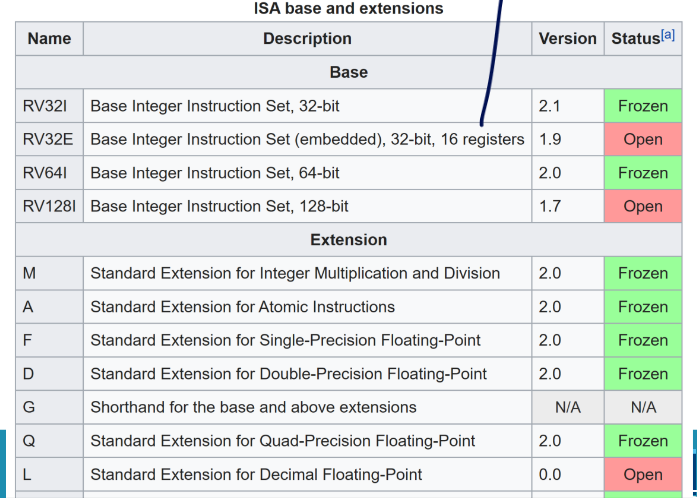
\includegraphics[width=0.55\linewidth]{RISCV_extensions.png}
    \caption{RISC-V Extensions}
    \label{fig:riscv-extensions-label}
\end{figure}

\subsection{Multiplier example}

If we are taking the example of the multiplier, we can't simply use \verb|mul t2, s1, s2| since multipling $N$ bits with $N$ bits will give us a $2N$ bits number. So we need to multiply the LSB first then MSB.

\begin{lstlisting}[language={[x86masm]Assembler}]
mul r0, r1, r2      ; multiply 32 bits with 32 bits store the LSB of 64 bits results in a 32 bits register
mulh r0, r1, r2     ; multiply 32 bits with 32 bits store the MSB of 64 bits results in a 32 bits register
mulhu r0, r1, r2    ; multiply 32 bits unsigned with 32 bits unsigned store the MSB of 64 bits results in a 32 bits register
mulshu r0, r1, r2   ; multiply 32 bits signed with 32 bits unsigned store the MSB of 64 bits results in a 32 bits register
\end{lstlisting}

We can also modify the datapath for multiplier for example if it doesn't meet the timing criteria. We can make it span over the ALU and memory read since we don't need to use a multiplier for load or store operation (only reason why ALU is before a memory access).\\

We can also think about variable length pipeline to make some instructions run more longer than other but we will run into collision problems. We can use some dynamic scheduling for this.

This type of exercise will be the same at the exam !
\chapter{The memory hierarchy}

The biggest bottleneck in modern computer is the time access of RAM. The larger the memory the slower it will since we will have higher capacitance due to the interconnect.

\begin{table}[h]
    \centering
    \begin{tabular}{lccc}
        \toprule
        \textbf{Memory Type} & \textbf{Location} & \textbf{Access Time} & \textbf{Cost per GB} \\
        \midrule
        Registers (flip-flops) & On-chip & $\leq$ 0.1 ns & - \\
        Static RAM (SRAM) & On-chip & $\sim$1 ns & $\sim$ \$1000 \\
        Dynamic RAM (DRAM) & Companion chip & $\sim$50 ns & $\sim$ \$10 \\
        Flash (SSD) & External storage & $\sim$10 $\mu$s & $\sim$ \$1 \\
        Magnetic disk (HD) & External storage & $\sim$1 ms & <\$0.1 \\
        \bottomrule
    \end{tabular}
    \caption{Comparison of different memory types}
    \label{tab:memory_comparison}
\end{table}

Ideally we would have everything in a register but this is simply impossible. Even having everything in SRAM is not feasible. What we will try to do with \textit{memory hierarchy} is to not see this tradeoff. We will also use locality in this context.

\begin{figure}[H]
    \centering
    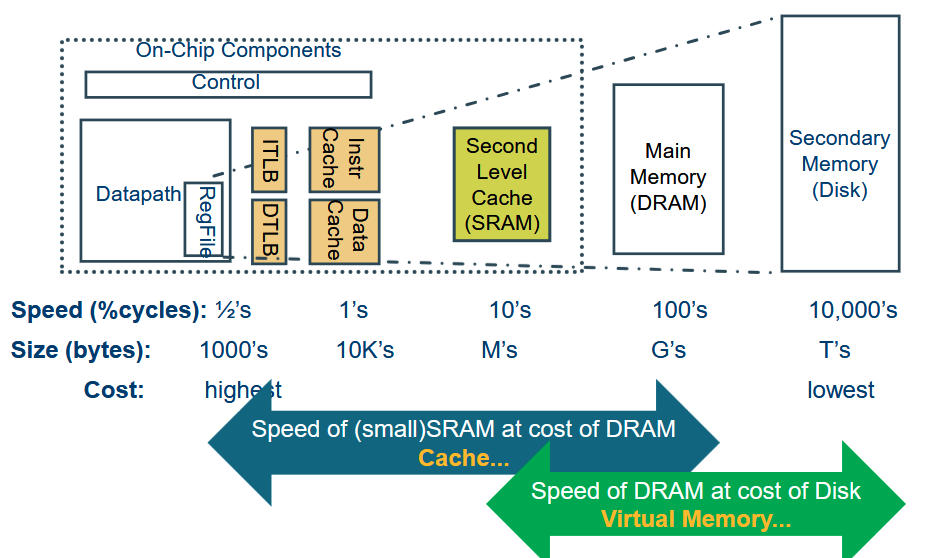
\includegraphics[width=0.75\linewidth]{Typical_memory.png}
    \caption{Typical memory hierarchy}
    \label{fig:enter-label}
\end{figure}

\section{Locality, caching and virtual memory}

There is two type of locality : 

\begin{enumerate}
    \item \underline{Temporal :} if a memory location is referenced, then it will tend to be referenced again soon. So we keep the most recently accessed data items.
    \item \underline{Spatial :} if a memory location is referenced, the neighboring locations tend to be referenced afterwards so we will load to full block of contiguous words.
\end{enumerate}

If we want to access something that isn't in the memory, we will have what we call a \textbf{miss}. We will have to get the data from a higher level memory location (SRAM, SSD, HDD, ...). That time that is lost to access the data is called the \textbf{miss penalty} and the amount of misses is called the \textbf{miss ratio} (MR = 1 - hit ratio).
If the data was in the cache we have a \textbf{hit}.

\section{Caching basics (recap)}

Cache is the closest memory to the CPU and the data are not always ordered. We need some sort of scheme to understand and know which data are present or not.

\subsection{Direct mapped cache}

We use the LSB of the addresses as the location in the cache. So we do block address modulo the amount of blocks in cache. The amount of block needs to be a power of 2.
Then we can use some validity bits and tag (MSB of the address) to know exactly what data is stored and if they are valid.

Here if we try to access the data 11010, we can see the tag doesn't match so it will result into a miss and we will most likely replace the 10010 data.


\begin{table}[h]
    \centering
    \renewcommand{\arraystretch}{1.3}
    \begin{tabular}{|c|c|c|c|}
        \hline
        \textbf{Index} & \textbf{V} & \textbf{Tag} & \textbf{Data} \\
        \hline
        000 & Y & 10 & Mem[10000] \\
        \hline
        001 & N &  &  \\
        \hline
        \textbf{\textcolor{red}{010}} & \textbf{\textcolor{red}{Y}} & \textbf{\textcolor{red}{10}} & \textbf{\textcolor{red}{Mem[10010]}} \\
        \hline
        011 & Y & 00 & Mem[00011] \\
        \hline
        100 & N &  &  \\
        \hline
        101 & N &  &  \\
        \hline
        110 & Y & 10 & Mem[10110] \\
        \hline
        111 & N &  &  \\
        \hline
    \end{tabular}
    \caption{Cache Table Representation}
    \label{tab:cache_table}
\end{table}

So if we want to store some words (4 bytes) we will work with 32 bits addressees. The LSB of 2 are not used since we want to access a full word. Then we can have a cache of $2^{10} = 1024$ entries, we will use the $32-2-10 = 20$ as the tag. On top of those $32+20$ bits of information to store we also need an extra bits for validity. So at the end the cache size needs to be $(1+20+32)\cdot(2^{10}) = 54272 \text{ bits} = 13568 \text{ bytes}$.\\

When we will store some data, there is two main strategies to update the cache and the main memory : 

\begin{itemize}
    \item \underline{Write through :} update in the cache and in memory. \textbf{Write miss} : write allocate : fetch the block and then perform as for a write hit. \textit{write around} : don't fetch the block just write in cache (good for initialization in program)
    \item \underline{Write back :} update only the cache. Add a \textit{dirty bit} which shows if the data has been modified. Implemented a sub-routine to update from the cache the memory. \textbf{Write miss} : just fetch the block and update it.
\end{itemize}

\section{Measuring cache performance Impact}

We want to quantify and be able to compare various algorithm to see what is the best for us in a given case or for a given application.

When we have a cache hit, nice everything goes as smoothly. But if we have a \textit{cache miss} we need to \textbf{stall} the CPU pipeline, fetch the block with the desired data from higher level hierarchy. But we can also have cache miss on \textit{CPU instructions} in which case we need to fetch until we get the right instruction.

We remember eq. \ref{eq:fundamental_perf}, we can simplify it with :

\begin{equation}
    \text{CPU time} = IC \cdot CPI \cdot \text{clock cycle time}
\end{equation}

And now our \textit{CPI} needs to take into account the \textit{program execution cycles} (add the possible cache hit time) and the time where we need to \textit{stall the pipeline} (memory stall cycles) to get the data.

\begin{equation}
     \text{Memory stall cycles} = \underbrace{\frac{\text{memory accesses}}{IC}}_{\text{How many time per instruction is it accessed}} \cdot \overbrace{\text{Miss rate}}^{miss/access} \cdot \underbrace{\text{Miss penalty}}_{\text{Clock cycle to wait}}
\end{equation}

From now on we will differentiate the cache for the instructions with \textbf{I-cache} and the cache for the data \textbf{D-cache}. With this we can separate and have various strategies depending on the type of cache.

There is also other interesting metrics such as the Average Memory Acess Time (AMAT) :

\begin{equation}
    AMAT = \text{Hit time } + \text{ Miss rate } \cdot \text{Miss penalty} 
\end{equation}

To reduce AMAT, we can reduce \textit{hit time}, reduce \textit{miss rate}, reduce \textit{miss penalty}\footnote{More detailed for reference – H\&P B.7}.

\section{Cache optimizations}

\subsection{Source of Misses}

\begin{itemize}
    \item \underline{Compulsory misses :} First access to a block. Typically at initialization time
    \item \underline{Conflict misses :} In a non-fully associative cache. Due to competition for entries in a set. Would not occur in a fully associative cache of the same total size. This \textbf{is not a space issue} but an issue with a set. If we change the amount of set we could avoid this error.
    \item \underline{Capacity misses :} Due to finite cache size. A replaced block is later accessed again (as it would be in fully associative cache)
    \item \underline{Coherence misses :} Miss because other processor has invalidated the cache line. Due to a store or manipulation, ...
\end{itemize}

\subsection{Basic}

\begin{table}[h]
    \centering
    \renewcommand{\arraystretch}{1.3}
    \begin{tabular}{|p{4.5cm}|c|c|c|p{2.5cm}|}
        \hline
        \textbf{Optimisation} & 
        \textbf{\textcolor{red}{Hit Time}} & 
        \textbf{\textcolor{ForestGreen}{Miss Rate}} & 
        \textbf{\textcolor{blue}{Miss Penalty}} & 
        \textbf{Hardware Complexity} \\
        \hline
        0. split/unified I/D cache & & & & 0 \\
        \hline
        1. larger cache & - & + & & 1 \\
        \hline
        2. larger block size & + (or -) & & - & 0 \\
        \hline
        3. higher associativity & - & + (-) & & 1 \\
        \hline
        4. multi-level cache & & & + & 2 \\
        \hline
        5. read priority over write & & & + & 1 \\
        \hline
        6. no address translation \newline \textit{(see part Virtual Memory)} & + & & & 1 \\
        \hline
    \end{tabular}
    \caption{Cache Optimization Techniques}
    \label{tab:cache_optimisation}
\end{table}

\subsubsection{0. Split vs. unified instruction/data caches}

We either use the same cache for instructions and data (\textbf{unified}) or we can choose to split in two (\textbf{split}). Instructions have better locality than data since we mostly access them sequently and thus we can use some specific strategies. Split cache is mostly used at lowest level.

\subsubsection{1. Larger cache}

We can simply use larger cache so we will have less misses. But it will increase the hit time since we will have more interconnect and capacitance when loading the data in. It will consume more power (static \& dynamic) and will come at an increased cost. So we can only do this for shared or off-chip caches.

\subsubsection{2. Larger block sizes}

To avoid to always load data from the cache, we can increase the block size hoping the user will request data that are next to the currently accessed data. It take advantage of the \textit{spatial locality} principle. 

Increasing it will have its benefit up to a certain point. This equilibrium is different depending on the cache size but we can always observe a degradation for bigger blocks. This is due to the fact we will quickly saturate the memory with data that are not useful for the user (\textit{pollution}). So this will simply \textit{increase the miss rate}.

We will also have a bigger miss penalty since we load more data. We can use \textit{early restart} and \textit{critical-word-first} to help with this problem.

\begin{figure}[H]
    \centering
    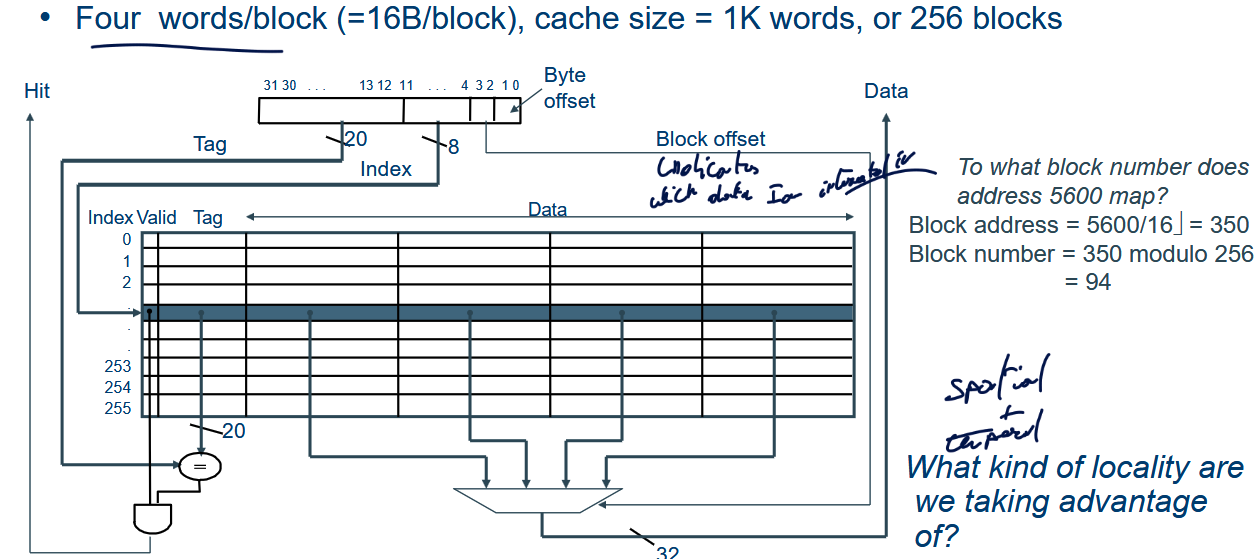
\includegraphics[width=0.85\linewidth]{data_block.png}
    \caption{How data is done in practice}
    \label{fig:data-block-label}
\end{figure}

\subsubsection{3. Higher associativity}

\begin{itemize}
    \item Full associativity : any block can go anywhere in cache
    \item Set associative : a block can only go to a set of the cache
    \item Direct mapped : a block can only go to a specific place of the cache
\end{itemize}

To describe the amount of sets, we are talking about \textbf{N-way set associative}. Where for N blocks of cache, N-associative correspond to \textit{full associativity} and 1-associative to \textit{direct mapped}.

To do full associativity we need to be able to search the whole cache and use \textit{comparator} per entry ! When using sets we can reduce the amount of comparator and reduce the search space. 

\begin{figure}[H]
    \centering
    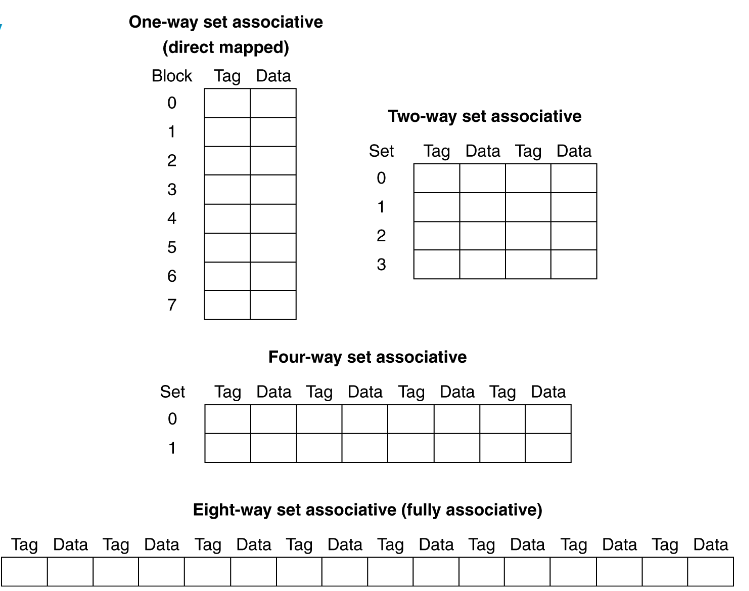
\includegraphics[width=0.5\linewidth]{set_associativity_cache.png}
    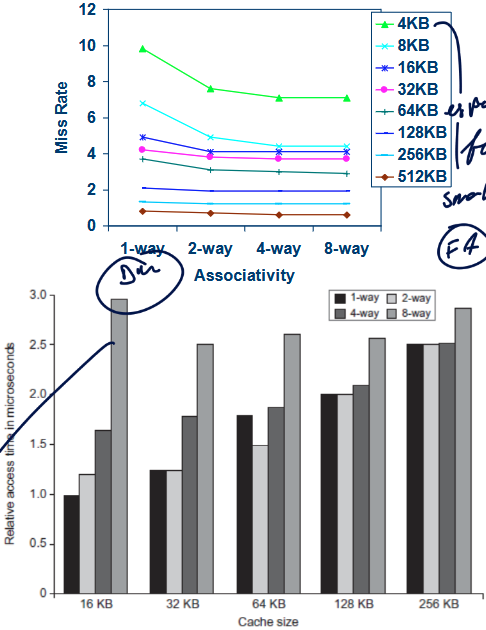
\includegraphics[width=0.4\linewidth]{perf_set_associativity.png}
    \caption{Set associativity represented in cache}
    \label{fig:set-asso-label}
\end{figure}

We can see that increasing the associativity will decrease the miss rate up to a certain point where we have little gain. On the other hand, we need extra logic and comparators ($n$). If we are comparing at equal gate amount, we will have less cache. The hit time is also slightly increased since we need to test every spot.

\begin{figure}[H]
    \centering
    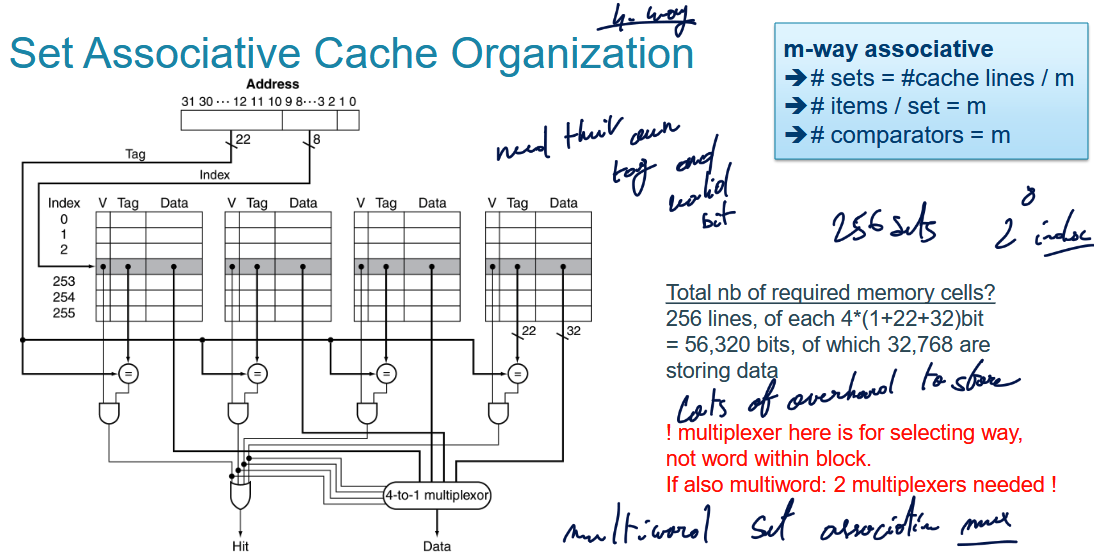
\includegraphics[width=0.75\linewidth]{set_associative.png}
    \caption{Set associativity implementation}
    \label{fig:set-associativity-impl-label}
\end{figure}

For direct mapped, the replacement policy is pretty straightforward, we will simply update the spot. For set associativity we will first remove non-valid entry and then check other candidate based on 3 different approach : 

\begin{enumerate}
    \item \textbf{Least-Recently Used (LRU) :} we will remove the data that was accessed a long time ago. For 2-way it is simple, 4-way it gets trickier and then it becomes just too hard.
    \item \textbf{FIFO :} we simply delete the oldest block, but it is inferior to LRU since we can have a block where we loop on it and use it all the time.
    \item \textbf{Random :} delete one randomly. The performance is pretty similar to LRU for high associativity which is a good thing !
\end{enumerate}

\subsubsection{4. Multi-level caches}

The idea is to have cache for cache. We will have smaller and smaller cache closer to the CPU. Those smaller caches are \textit{low associative} to have better speed performance but will have larger miss rate with a small block size. For second level, we will try to minimize the miss rate we need larger cache, higher associativity, larger block size.

We often denote those caches like $1\$$ or $2\$$, when in an exercise we give the hit rate, we are always talking with \textbf{local rate} so from $1\$$ to $2\$$ and not from the processor to the $2\$$. So how to compute the \textit{AMAT} ?

\begin{equation}
    AMAT = \text{hit time L1} + \text{miss rate L1} \cdot (\text{hit time L2} + \text{miss rate L2}\cdot \text{miss penalty L2})
\end{equation}

So we simply need the local misses from one level to the other. By using this formula with some real example, we can see we can get much much closer to the ideal $1$ clock cycle for data access.

\begin{table}[H]
    \centering
    \begin{tabular}{|c|p{1.6cm}|p{1.6cm}|p{1.6cm}|p{1.6cm}|p{1.6cm}|p{1.6cm}|}
        \hline
        \textbf{hit rate} & \textbf{L1 and main} & \textbf{L1, L15 and main} & \textbf{L1, L10, L20 and main} & \textbf{L1, L3, L10, L20 and main} & \textbf{L1, L3, L5, ..., L19, main} & \textbf{all levels} \\
        \hline
        100.00 & 1.00  & 1.00  & 1.00  & 1.00  & 1.00  & 1.00  \\
        99.00  & 1.50  & 1.16  & 1.10  & 1.03  & 1.03  & 1.02  \\
        98.00  & 2.00  & 1.32  & 1.21  & 1.06  & 1.06  & 1.04  \\
        97.00  & 2.50  & 1.50  & 1.32  & 1.10  & 1.09  & 1.06  \\
        96.00  & 3.00  & 1.68  & 1.44  & 1.14  & 1.13  & 1.09  \\
        95.00  & 3.50  & 1.88  & 1.56  & 1.18  & 1.16  & 1.11  \\
        90.00  & 6.00  & 3.00  & 2.25  & 1.43  & 1.36  & 1.23  \\
        80.00  & 11.00 & 6.00  & 4.20  & 2.24  & 1.87  & 1.56  \\
        70.00  & 16.00 & 10.00 & 7.15  & 3.75  & 2.65  & 2.04  \\
        60.00  & 21.00 & 15.00 & 11.40 & 6.36  & 3.89  & 2.79  \\
        50.00  & 26.00 & 21.00 & 17.25 & 10.63 & 5.99  & 4.06  \\
        \hline
    \end{tabular}
    \caption{Hit Rate vs. Cache Levels Performance}
    \label{tab:hit_rate_performance}
\end{table}

\subsubsection{5. Prioritize reads over writes}

In this optimization, we will have a \textit{write buffer} and a read miss will stall the processor. We don't want a write to stall the processor even though they may take quite some time to complete. To evict a dirty block for a read, we can copy dirty block to write buffer and immediately proceed to read data. 

In \textit{write through}, we will let the processor write to the buffer and then it will be written to $2\$$ cache. For \textit{write back}, we will let the $1\$$ cache write to the buffer and then a sub-routine will copy this data to the $2\$$ cache.

\subsection{Advanced}

\begin{table}[H]
    \centering
    \begin{tabular}{|p{2.1cm}|p{1.8cm}|p{1.8cm}|p{1.8cm}|p{1.8cm}|p{1.8cm}|p{1.8cm}|}
        \hline
        \textbf{optimisation} & \textbf{\textcolor{red}{hit time}} & \textbf{bandwidth} & \textbf{\textcolor{green}{miss rate}} & \textbf{\textcolor{blue}{miss penalty}} & \textbf{power consumption} & \textbf{hardware complexity} \\
        \hline
        1 way-predicting &  & + &  & - & + & 1 \\
        2 pipelined & + (but multicycle) &  &  &  &  & 1 \\
        3 multi-banked &  & + &  &  &  & 2 \\
        4 non-blocking &  & + &  & + &  & 3 \\
        5 critical word first \& early restart &  &  &  & + &  & 2 \\
        6 merging write buffer &  &  &  & + & - & 1 \\
        7 (HW or SW) prefetching &  &  & + & + &  & 2/3 \\
        8 compiler optimizations &  &  & + & + &  & 3 \\
        \hline
    \end{tabular}
    \caption{Cache Optimization Techniques and Their Effects}
    \label{tab:cache_advanced_optimizations}
\end{table}

\subsubsection{1. Way prediction}

We will try to load the next access and pre-set the mux since there is a lot of logic on the way from the tag to the data out. If we miss, it will cost more time so increasing the hit time but the accuracy is quite good, $>90\%$ for two-way and $>80\%$ for four-way. We got better accuracy for I cache than D cache. It will still consume a lot of power since we may access unwanted slice so we will put some cell into sleep mode.

\subsubsection{2. Pipelined caches}

It is to clock the CPU even faster than the L1 cache access time. But this will increases the branch mis-prediction penalty and we can easily increase associativity since it's not too bad to slow down the cache now.

\subsubsection{3. Multi-banked caches}

To read efficiently, we will try to read with a \textit{single port} but we could have \textit{simultaneous} read access for shared cache.

\textbf{READ MORE THIS PART CAUSE I DONT UNDERSTAND IT}

\subsubsection{4. Non-blocking cache}

In an \textit{in-order} processor, the cache miss will result into a \textit{processor stalls} so we simply have to wait until we get the data back. With an \textit{out-of-order} processor, we can do other instructions while waiting for previous ones.

We won't stall when we get a load instructions and will simply keep running other independent instructions. But if we have other load instructions, we could still stall if we are encountering blocking or non-blocking cache. 

With non-blocking cache, we will not stall but still service other memory requests. We can have hit before previous misses complete "\textit{hit under miss}", "\textit{hit under multiple miss}" but also stall with "\textit{miss under miss}". We have blocking L2 cache which will not hide the miss penalty sadly. But this has its fair bit of problems : 

\begin{itemize}
    \item multiple outstanding misses: keep track which instruction asked for it
    \item arbitration between outstanding requests: L1 hits can collide with misses returning from L2. Multiple misses returning from L2 can collide when mapped to the same block. L2 data can return out of order
\end{itemize}

\subsubsection{5. Critical word first, early restart}

This method is applicable for caches with block size bigger than 1 upon cache miss. We start with the critical word first. Request missed word from memory first then we send it to the processor as soon it arrives.

For early restart,  we request words in normal order and we send the missed work to the processor as soon as it arrives. The effectiveness of these strategies depends on the block size and likelihood of another access to the portion of the block that has not yet been fetched.

\subsubsection{6. Merging write buffer}

When we store to a block that is already pending in the write buffer, we update the write buffer. It reduces the stalls due to a full write buffer and reduce write buffer entries.

\subsubsection{7. Prefetching}

We request the data from the cache before it is actually needed. So we give the time to the cache to handle a miss by the time the data is needed. We will have longer lifetime of the data in the cache and we could interfere with other previous memory accesses which would have worse performance.

We can do it in HW which is usually done for L1 cache but it requires more hardware. But we can also do it in software (through the compiler or the programmer itself). We can do some loop unrolling or prepare some load and pipeline the software. It will requires thus a bit more instructions.

\subsubsection{8. Other compiler optimizations}

Typically, we can do some better matrix and array access. For example, since we know we will load a full row in the cache, instead of accessing the elements from top to bottom, we can decide to access from left to right. This will increase the hit rate since we will load in memory the full row when accessing the first entry. We can do some \textit{loop inversion}.

If the row is too big to be loaded in cache, memory, ... we can do \textit{tiling} where we will break down a loop into smaller pieces. It will have a better locality, and it usually looks like this :

\begin{lstlisting}[language=c, caption=Typical tiling]
for (i1 = 0; i1 <= 1; i1 = i1 + 1)
    for (j = 0; j < N; j = j + 1)
        for (i2 = 0; i < N/2; i2 = i2 + 1){
            i = N/2*i1+i2;
            z[i][j] = z[i-1][j] + x[i][j]*y[i][j];
        };
\end{lstlisting}

\section{Virtual machines and virtual memory}

In this paradigm, we explore the idea of having the speed of DRAM with the space of a disk. Even 32 GB of RAM is not always enough to run every program all at once and OS's have developed technique to put unused software in standby and to free up ram.

We know that all of the programs, files, ... are stored on a \textbf{secondary memory} called disk space. And when we run a program we would like to load the full program to be able to run it and exploit it. But this is not always feasible, so we will use a \textbf{swap space} that is a sort of extension of the ram into the disk space. But this requires a better \textit{book keeping} for the OS to know which piece of code is in ram or not. We need a good management unit.

\subsection{Virtual memory}

We use the memory as a cache for the secondary storage. We are going to use clean, stable and unified addresses that are both managed by the CPU and the OS. The virtual address space is \textbf{larger than} the physical address space, we give the illusion of an infinite ressource.

The processor will work with virtual memory that is contiguous and unified from his POV. Those virtual memory addresses will get automatically translated into physical one later. Easier to develop an application since we don't need to think how it will be managed in memory. Makes it more secure with isolation processes and can give more ressources than actual present on the machine by using swap.

\subsubsection{Page}

We call a virtual memory block a \textbf{page}. Usually they contain multiple addresses and we will use this as the \textit{page offset}.

\begin{figure}[H]
    \centering
    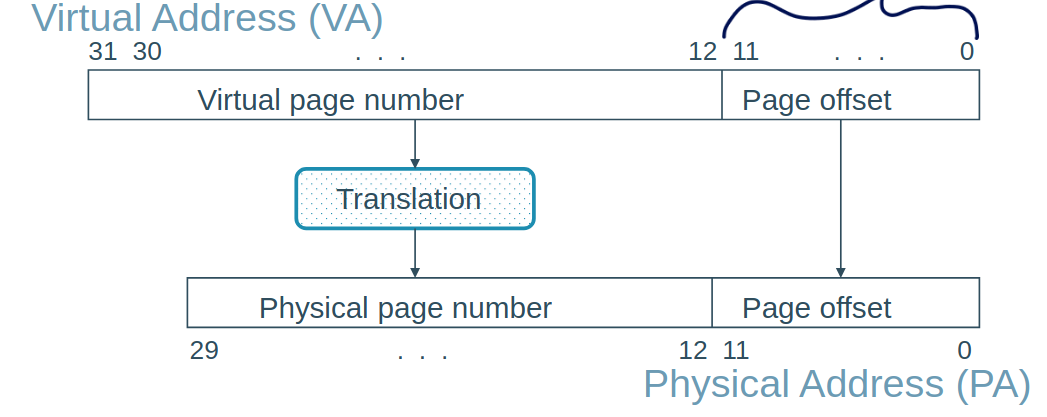
\includegraphics[width=0.75\linewidth]{translation_VM.png}
    \caption{Translation of VA}
    \label{fig:translation-va-label}
\end{figure}

There is a LUT that is stored in memory that helps with the translation of the VA into physical one. There is only one page for each process and they form with the program counter and register the current state of a program. When starting a new process, the operating system simply loads the page table register to point to the page table of the process it wants to make active (and loads the register file and the program counter)

\begin{figure}[H]
    \centering
    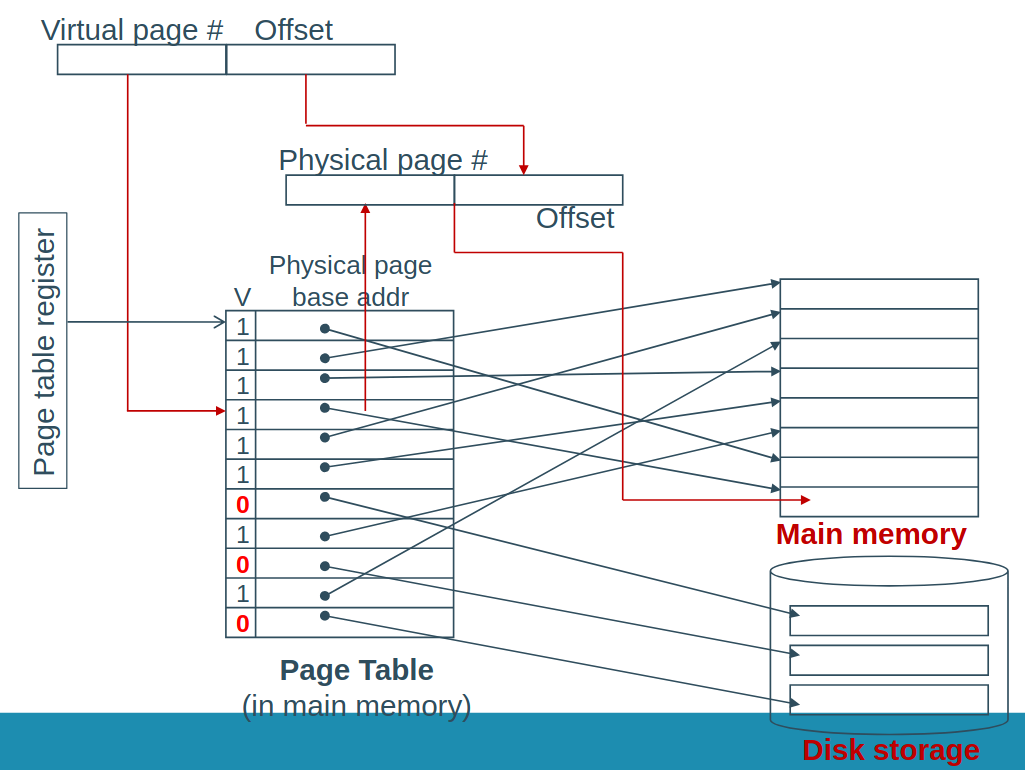
\includegraphics[width=0.75\linewidth]{TLB_mechanism.png}
    \caption{Translation mechanism}
    \label{fig:tlb-label}
\end{figure}

\subsubsection{Page tables}

It stores the placement information and is an array of page entries that we index by virtual page number. Page table register in CPU points to page table in physical memory. If a page is present in memory, the \textit{page table entry} will store the physical page number. We will also add dirty bit and reference bit.

When we have a \textit{fault}, we need to look into the swap space, this is handled by the OS and takes \textit{millions} of CPU cycles. That's why we need smart replacement algorithms and fully associative placement of pages in main memory.

\subsubsection{Replacement}

The ideal algorithm is the LRU but hard to keep track of all access and updating it, too costly. We will use the \textit{reference bit} algorithm where we set to 1 when it has been accessed. The OS will \textit{periodically} clear those bits to put them back to 0. When we need to do replacement, we will first remove the one where their bit is 0.

\begin{figure}[H]
    \centering
    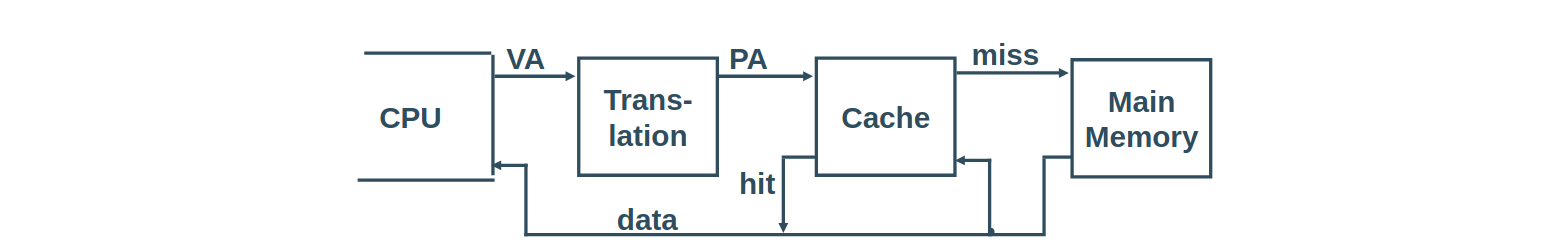
\includegraphics[width=0.95\linewidth]{cache_TLB.png}
    \caption{Cache in TLB}
    \label{fig:cache-tlb-label}
\end{figure}

This makes cache access pretty expensive,  that's why we are going to use a TLB for this purpose. This will make accessing memory much much faster. It is a pretty small with 19 to 512 entries.

\begin{figure}[H]
    \centering
    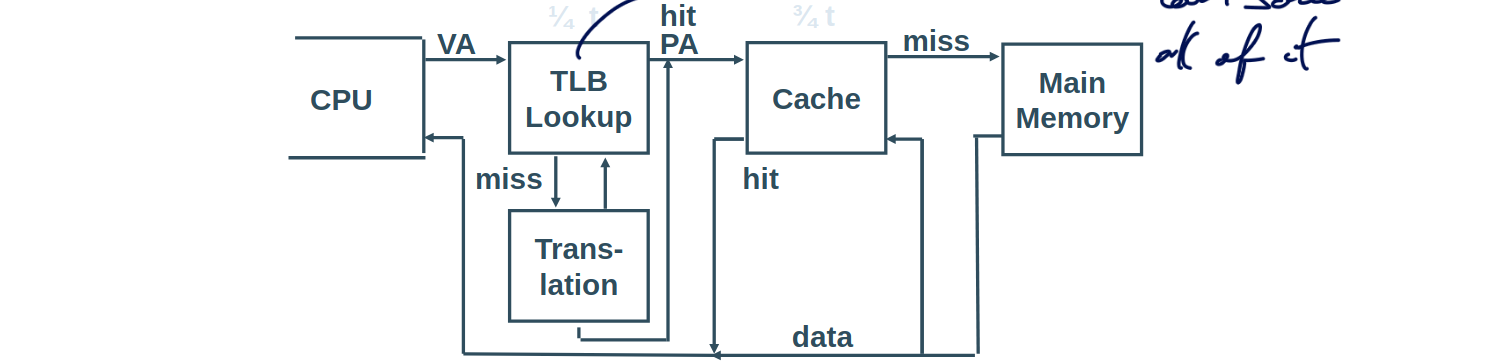
\includegraphics[width=0.95\linewidth]{TLB_hierarchy.png}
    \caption{Hierarchy TLB}
    \label{fig:hierarchy-tlb-label}
\end{figure}

If we have a TLB miss, we can either have the page loaded in memory and so we can add this entry into the TLB. But if it is not the case, we have a page miss which will have a higher penalty. Luckily, TLB misses are more frequent than total page misses.

\subsubsection{Why Not a Virtually Addressed Cache?}

A virtually addressed cache would only require address translation on cache misses. But with this idea, we can't do shared data. Since each process will have its own VA and so its own entry in the TLB. So modifying one data will force us to update the other one manually. Not that efficient in the end.

To reduce the translation time, we can overlap the cache access with the TLB access. It works when the high order bits of the VA are used to access the TLB while the low order bits are used as index into cache.

\begin{table}[H]
    \centering
    \begin{tabular}{|c|c|c||m{8cm}|}
        \hline
        \textbf{TLB} & \textbf{Page Table} & \textbf{Cache} & \textbf{Possible? Under what circumstances?} \\
        \hline
        \hline
        Hit & Hit & Hit & \textcolor{ForestGreen}{Yes} -- what we want! \\
        \hline
        Hit & Hit & Miss & \textcolor{ForestGreen}{Yes} -- although the page table is not checked if the TLB hits \\
        \hline
        Miss & Hit & Hit & \textcolor{ForestGreen}{Yes} -- TLB miss, PA in page table \\
        \hline
        Miss & Hit & Miss & \textcolor{ForestGreen}{Yes} -- TLB miss, PA in page table, but data not in cache \\
        \hline
        Miss & Miss & Miss & \textcolor{ForestGreen}{Yes} -- page fault \\
        \hline
        Hit & Miss & Miss/Hit & \textcolor{red}{Impossible} -- TLB translation not possible if page is not present in memory \\
        \hline
        Miss & Miss & Hit & \textcolor{red}{Impossible} -- data not allowed in cache if page is not in memory \\
        \hline
    \end{tabular}
    \caption{TLB, Page Table, and Cache Possibilities}
    \label{tab:tlb_page_table_cache}
\end{table}

\textbf{Up to page 103}

\section{Scratchpads and DMA}

Sometimes, we don't want this high level and virtualization and we want to access all of this at the Software level. If we know we will often reuse data, we want to better plan and better use the memory. 

Using cache is good for:

\begin{itemize}
    \item Non real time software, and no predictive data (aka, we can't have things arriving late and we can't do sw optimization)
    \item Cache used in GP CPU
    \item Easy to program with it
\end{itemize}

We shouldn't use cache for:

\begin{itemize}
    \item Hard real-time application with strict deadline (we can't have TLB miss or stuff like this)
    \item We can predict patterns and do better software programming
\end{itemize}

The idea behind \textit{scratch pad} is for the programmer to better plan the memory usage and be able to plan how his elements will be stored in memory. Heavily used in DSP where we have repetitive and fast processes.

\subsection{Direct Memory Access (DMA)}

Transferring data is taking a lot of time and we wouldn't want our precious CPU cycles to be wasted just moving data. That's why we have created the DMA which is a \textit{hardwired state machine}, its only goal is to store data, move data to memory or peripheral and back. It has its own subroutine and run in parallel to the CPU. 

\begin{figure}[H]
    \centering
    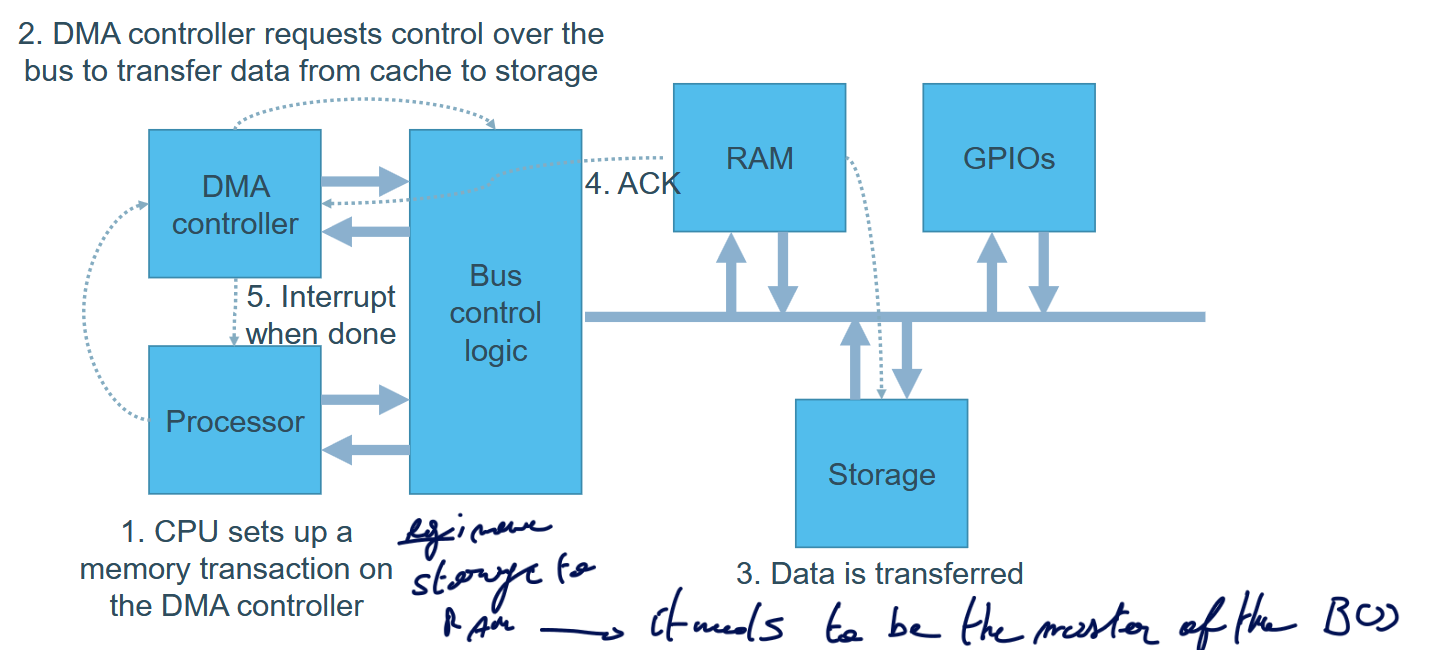
\includegraphics[width=0.75\linewidth]{DMA-controller.png}
    \caption{DMA controller}
    \label{fig:DMA-controller-label}
\end{figure}

\subsubsection{BUS arbitration}

We need to implement an algorithm to transfer the ownership of the BUS between peripherals. When we are done using the BUS through one peripheral, we let the ownership go and another device can take control.

This is implement with active low signal. It is in 4 phases

\begin{enumerate}
    \item DMAC request BUS with $\overline{BR}$
    \item $\mu P$ finishes its current operations and grand the bus through $\overline{BG}$
    \item DMAC starts controlling and releases the BUS and releases $\overline{BR}$.
    \item $\mu P$ releases $\overline{BG}$ and gets the control of BUS.
\end{enumerate}

\begin{lstlisting}
WHILE 1
    WHILE StartDMA=0;
    BR' := 0;
    WHILE BG'=1;
    WHILE Nr > 0
        Out := Mem[StartAddress+Nr];
        || Nr := Nr -1;
    BR' := 1;
    WHILE BG'=0
\end{lstlisting}

\begin{table}[H]
    \centering
    \begin{tabular}{|c|p{3,5cm}|p{3,5cm}|p{3,5cm}|}
         \hline 
        Method & Advantages & Disadvantages & Use\\
        \hline
        Burst mode DMA & just one time overhead, pages burst memory modes can be used & Processor is idle during long time & good for fast non-interruptable peripherals. Advanced processors with memory bottleneck and with advanced memory chips. \\
        \hline 
        Cycle stealing DMA & Memory BUS is not blocked for a long time & High overhead cause we need to renegotiate bus mastership often & Slow peripherals that would keep the DMA controller waiting between successive transfers. Low performance system where memory access is not a bottleneck.\\
        \hline
    \end{tabular}
    \caption{DMA method}
    \label{tab:my_label}
\end{table}

\section{Memory technologies}

\begin{itemize}
    \item \underline{SRAM:} We can't physically have more L1 cache since it is using 6 transistor cells to store one bit, we have a low density. Moreover, it is expensive and high power but will keep data on forever until it is powered off. Fast $1ns$
    \item \underline{DRAM:} High density only 1 transistor per cell, requires low power and cheaper. Needs to be refreshed (every $\sim 8ms$). Pretty slow $50 ns$.
    \item \underline{HDD/SSD:} pretty slow but non-volatile.
\end{itemize}

\subsection{Memory array}

All the data in memory are agenced in an \textbf{array} like structure. Where we have \textit{wordline} controlled by the MSBs and the \textit{bitline} controlled by the LSBs.

\subsubsection{Read Only Memory (ROM)}

As the name suggests, it is a type of memory that can only be written, an absence of transistor is a 1 and a transistor is a 0. Good for Boot loader and critical component like those.

\begin{figure}[H]
    \centering
    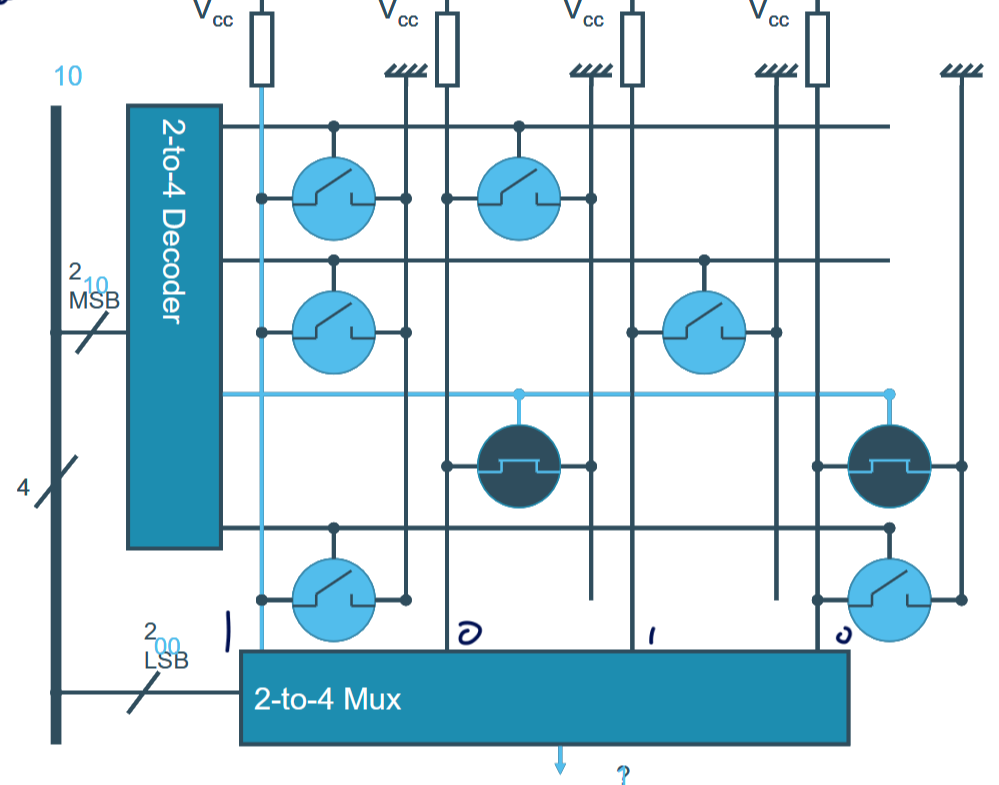
\includegraphics[width=0.4\linewidth]{memory_ROM.png}
    \caption{ROM}
    \label{fig:ROM-label}
\end{figure}

\subsubsection{Programmable ROM (PROM)}

Instead of only using a hardware specific ROM, we can link the gate of the transistors to the matrix with a fuse and when we want to write a program to it, we burn those fuses.

\subsection{SRAM}

\begin{figure}[H]
    \centering
    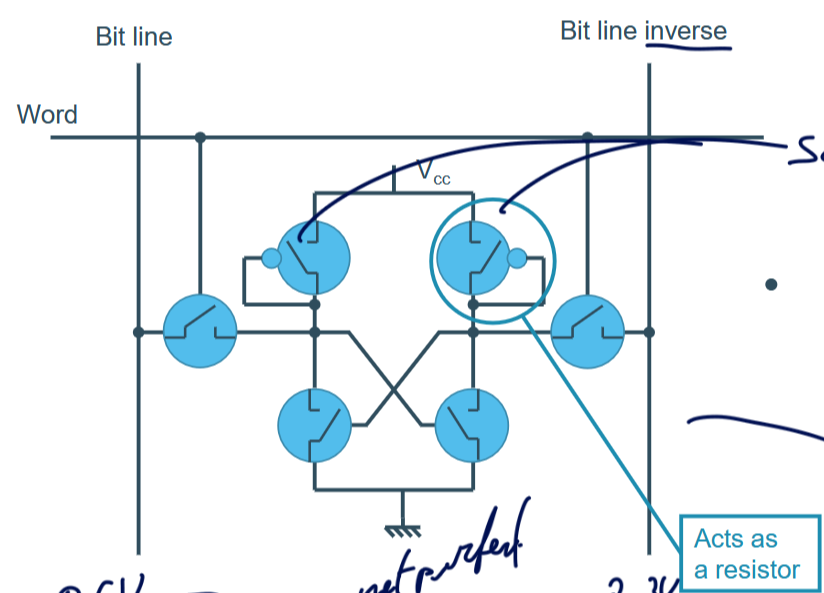
\includegraphics[width=0.5\linewidth]{SRAM-bitcell.png}
    \caption{SRAM bit cell}
    \label{fig:enter-label}
\end{figure}

It is basically a latch with two inverter and some nmos at the input to let and store the data.

As year progress, most of the area is used in a SOC by the cache and not really by new or re-used IP blocks.

\subsection{DRAM}

\begin{figure}[H]
    \centering
    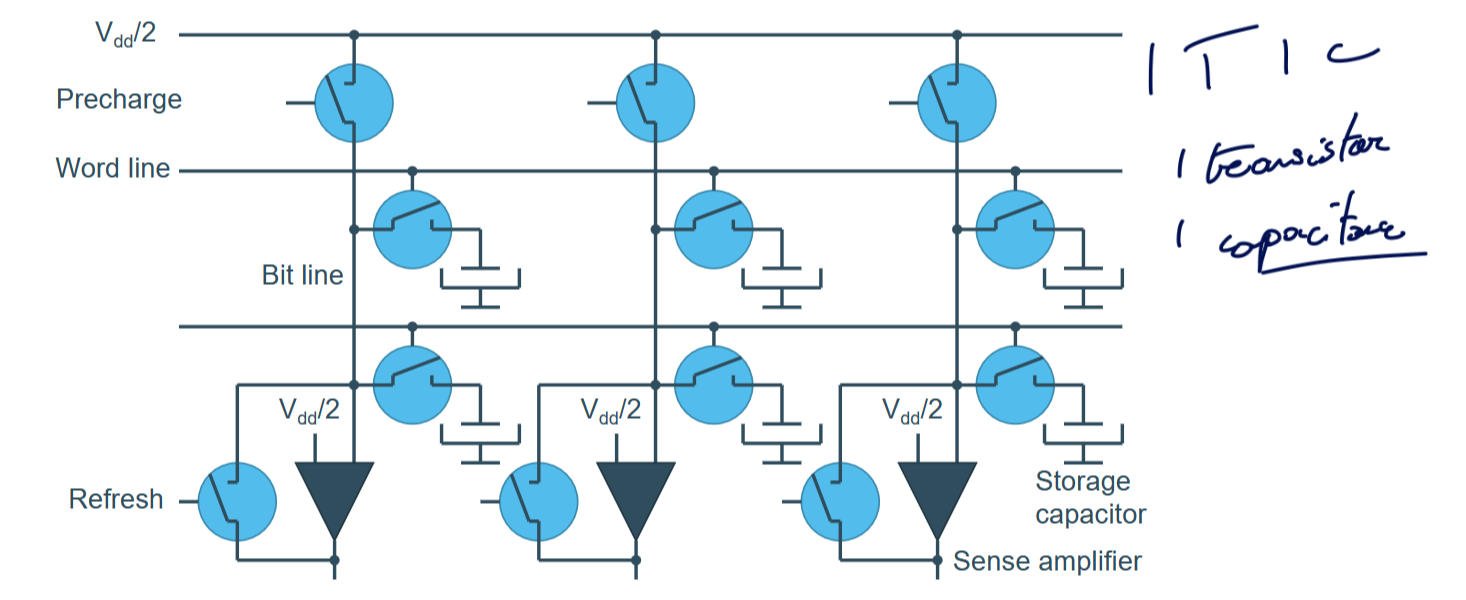
\includegraphics[width=0.75\linewidth]{DRAM-structure.png}
    \caption{DRAM structure}
    \label{fig:DRAM-structure-label}
\end{figure}

The capacitance are implemented vertically in the wafer to maximize their values while maintaining a high density as possible.

In DRAM, we need to precharge before doing a read or the values may not be read correctly. When we read, the values are slightly higher than $V_{DD}/2$ for a 1 bit and slightly below. It is pretty small difference that's why we need a comparator to check the value.

We read the full word line in DRAM. We then refresh the values after the comparator to reset the value that was read. Summary:

\begin{enumerate}
    \item Precharge
    \item Row Address Select: read all cells on a single wordline (destructive process)
    \item Sense comparator
    \item Column Address Select: we can be only interested in one bit for example
    \item Refresh: restor the content
\end{enumerate}

We must refresh after each read but also when the data is not used for quite some times since we have leakage on the capacitance.

\subsubsection{Processor Memory interface}

\begin{figure}[H]
    \centering
    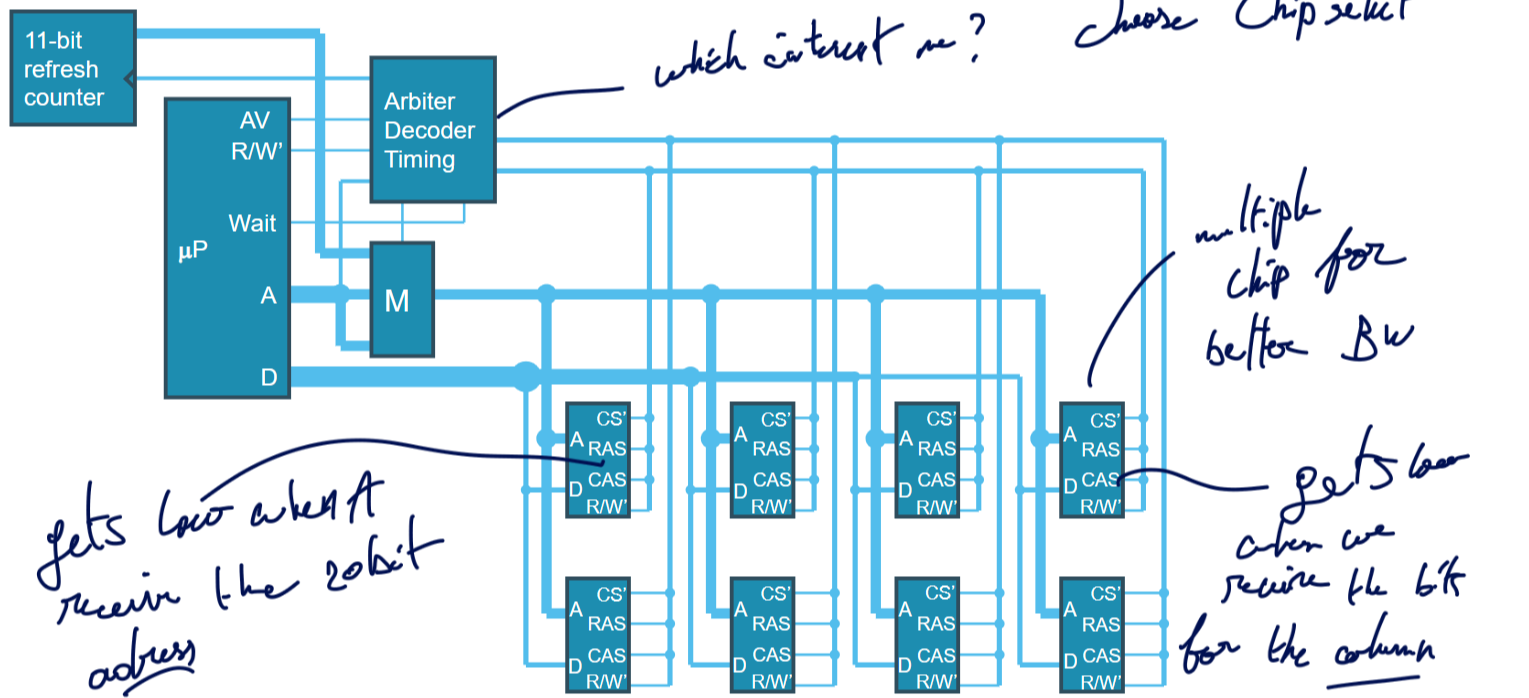
\includegraphics[width=0.75\linewidth]{interface_ram.png}
    \caption{DRAM interface}
    \label{fig:enter-label}
\end{figure}

In a RAM stick, there is multiple RAM chip so we first need to indicate which chip is of interest with chip select wire. Then we can specify the the CAS and RAS. But this process is quite slow so we spent lot of efforts to make this process quite faster.

\subsubsection{SDRAM}

\begin{figure}[H]
    \centering
    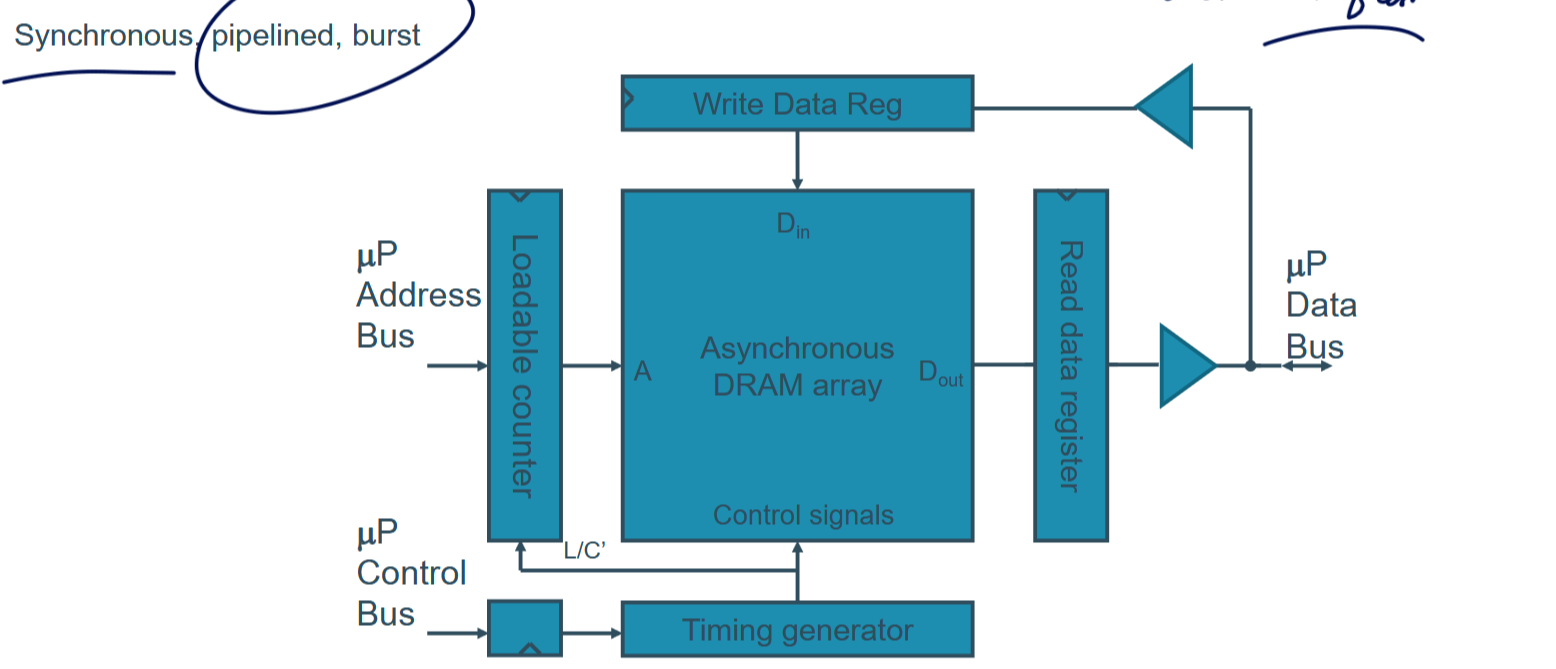
\includegraphics[width=0.75\linewidth]{SDRAM.png}
    \caption{Synchronous, pipelined, burst}
    \label{fig:SDRAM-label}
\end{figure}

It allows us to pipeline and so operate at a slightly faster rate. We can also use some \textit{bank interleaving} so we can use one bank and wait for another to precharge etc.

\subsubsection{DDR}

One of the most recent and paradigm that gets update regularly is the Double Data Rate scheme where we can read on the rising and the falling edge. So we can have a faster internal clock. This method assumes consecutive words to realize this technique.

\subsubsection{Stacked packaging}

In ARM and more efficient processor, we are stacking the memory on the same die or just nearby. We are talking about 3D DRAM if we stack it directly on top of the CPU die (quite challenging to do), or 2.5D DRAM if we put that stack DRAM just next to the CPU die.

Most high level caches are becoming eDRAM, especially seen in IBM server processor but still experimental.

\chapter{Exploiting Instruction Level Parllelism (ILP)}
\label{part-3}

\section{The roofline diagram}

It is a type of diagram that is used to evaluate and compare various solution for a given task.

We first start analyzing and checking how many useful operation per second can a given processor execute. This metric is given in GFLOP/s:

\begin{equation}
    Peak= f_{clk} \cdot op/clock \text{ } cycle \qquad IPC = instruction/cycle = 1/CPI
\end{equation}

We know a system is then constrained by its memory bandwidth, so we can draw a line indicating how constrained it is. This line is expressed in bytes per second.

The graph has the \textbf{Arithmetic Intensity} as its x axis, it indicates the ratio of operation per byte. So it is easy to know looking at the roofline graph if we are communication constrained or computational constrained.

Analyzing such graphs can quickly transmit a lot of information about a system and helps us creating the best one possible. Ideally, we want to be at the cut-off to avoid any waste.

\section{Tricks and limitations of static ILP}

One way to enhance and run more instructions per second is using static ILP. It is the compiler's responsibility to compile properly the instruction and to distribute the load. So, we need to compile for each and every possible platform. It is not a one fits all solution.

We call this a \textbf{Very Large Instruction Word}, because if we have 4 processors for example running at 32 bits, we will get some 128 bits instruction ! So the IPC > 1 and the CPI < 1.

\subsection{Issues}

Typically, in such processors they won't all run the same instructions, we can have some dedicated processor for operations.

One other challenge is that those type of processors are not always efficient for every program. Typically, we need high parallelism and avoid data dependency to be able to gain from it.

The compiler can't decide for the programmer so it is up to the programmer to be smart.

\subsubsection{Overcoming}

One good way to overcome this is by using \textbf{loop unrolling} and \textbf{predication}. We can optimize \textit{basic blocks}\footnote{Sequence of instructions with no embedded branches or branch targets}.

But also, hardware designer try to optimize their hardware for frequent use cases such as for loops. Indeed, it is not always smart to always increment a variable in a predictive manner. We are losing a precious clock cycle. So they came up with a better idea:

\begin{lstlisting}[language={[RISC-V]Assembler}]
    lp.setupi   100, Lend
    lw          x2, 0(x10)
    addi        x10, x10, 5
    addi        x2, x2, 1
    sw          x2, 0(x11)
Lend: addi      x11, x11, 4
\end{lstlisting}

So here, it will update the counter before the instructions memory.

Another way to optimize is to use some \textbf{guarded execution using predicates}. Instead of doing a conditional jump and so breaking a basic block, we will make the two condition execute and only write back after evaluation:

\begin{lstlisting}[language={[RISC-V]Assembler}]
r1 = 10;
r2 = A[r1];
r7 = (r2 > 0);
(r7) r3 = r3 + r2;
(r7)` r3= r3 - r2;
r5 = r4 - r3;
r6 = r3 + r4;
\end{lstlisting}

To use this extension, we need to support conditional write.

\begin{figure}[H]
    \centering
    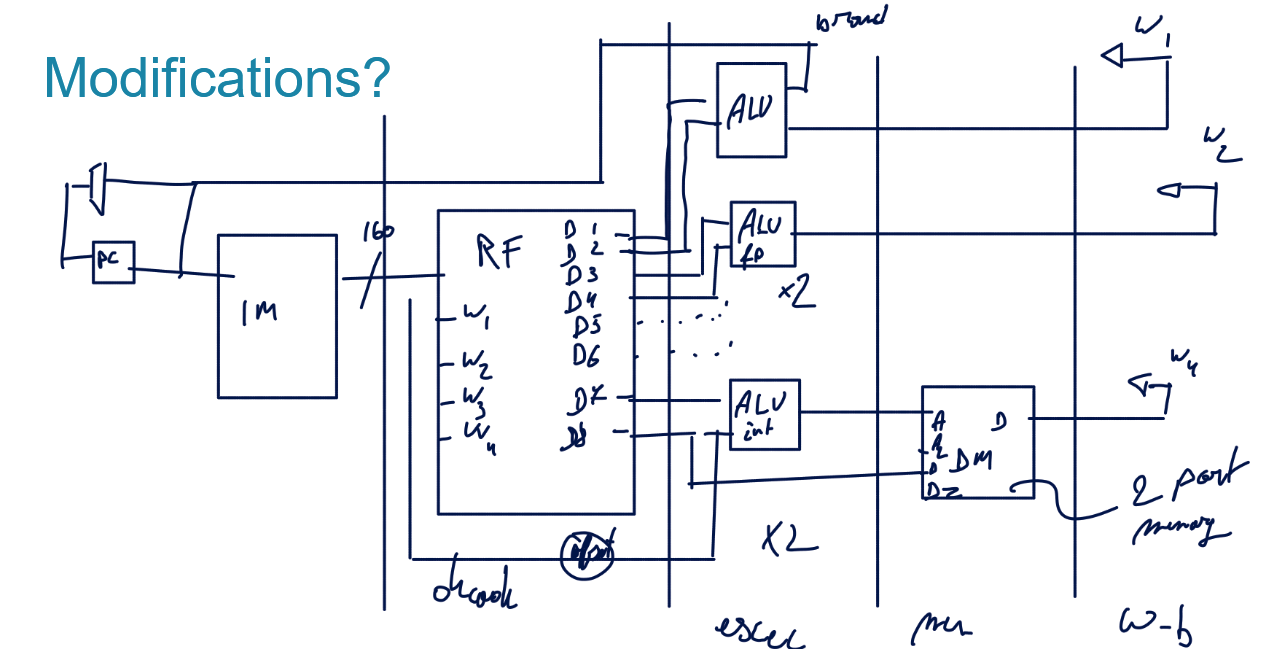
\includegraphics[width=0.75\linewidth]{multiple_issue_VLIW.png}
    \caption{Example with 1 integer instruction, 2 FP operations, 2 memory operations}
    \label{fig:VLIW-label}
\end{figure}

\subsection{Pipelined processor performance}

The hazard limit processor performance, we want more IPC but only possible in static schedule so we must optimize accross branches.

\subsection{Summary}

\begin{itemize}
    \item Yet, needs large “basic block size” to shuffle instructions around (gives degrees of freedom to compiler)
    \item Loop unrolling and predication (and later SIMD, see Part 4) help, but...
    \item Remaining challenges:
    \begin{itemize}
        \item No code compatibility among different processors (each processor needs own compiler!)
        \item Even with all previous tricks, hard to prevent all stalls at compile time (missing run-time information)
    \end{itemize}
\end{itemize}

We would like rather to rearrange instructions on the fly to be more flexible and dynamic.

\section{Dynamic ILP and Tomasulo’s algorithm}

Here, the CPU is the master and no longer the compiler, he is in charge of dispatching the instructions. So we don't have to recompile for every platforms and flavors of an architecture. More flexible and dynamic so can handle dependencies unknown at compile time.

Come at the cost of more complex hardware.

Such CPU can run instructions in or out-of-order instructions. But we need to carefully handle data hazards

\subsection{Data hazards}

We have 3 types of data hazards that can be real one and ones that are due to the limited amount of available registers:

\begin{enumerate}
    \item \underline{\textbf{Read After Write:}} we have a \textit{true dependence} between data and some data are not directly accessible.
    \item \underline{\textbf{Write After Read:}}  we have an \textit{anti-dependence} due to reusing a register name we may overwrite before the previous instruction has run. Possible and problematic in out-of-order execution only!
    \item \underline{\textbf{Write After Write:}} we have an \textbf{output dependence} because we are reusing the same name. Only possible and problematic in out-of-order execution only! 
\end{enumerate}

\begin{lstlisting}[language={[RISC-V]Assembler}]
; RAW
    x2 <- x1 + x3
    x4 <- x2 + x3

; WAR
    x2 <- x1 + x3
    x3 <- x4 + x5

; WAW
    x2 <- x1 + x3
    x2 <- x4 + x5
\end{lstlisting}

\subsection{Principles}

\begin{figure}[H]
    \centering
    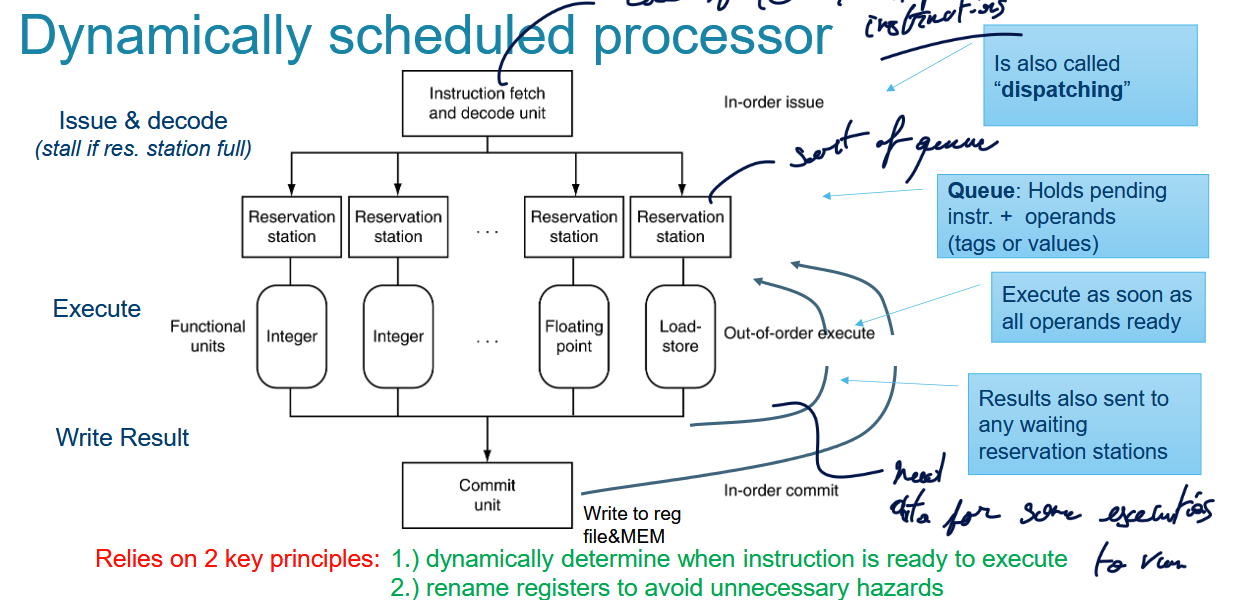
\includegraphics[width=0.85\linewidth]{dynamic_principle.png}
    \caption{Dynamically scheduled processor}
    \label{fig:dynamic_principle-label}
\end{figure}

To prevent WAW and WAR, we can do some registers renaming to avoid those false dependencies. But to do it on the fly we will use the \textbf{Tomasulo's algorithm} for it.

\subsection{Tomasulo's algorithm}

\begin{enumerate}
    \item \underline{\textbf{Issue (IS):}} we get the instruction from the instruction unit. If we have one reservation station free we issue an instruction and send operands.
    \item \underline{\textbf{Execute (EX):}} when both operands are ready we execute or we wait and monitor the Common Data Bus for result.
    \item \underline{\textbf{Write result (WR):}} write on Common Data Bus to all awaiting  units and mark the reservation station as available.
\end{enumerate}

\begin{figure}[H]
    \centering
    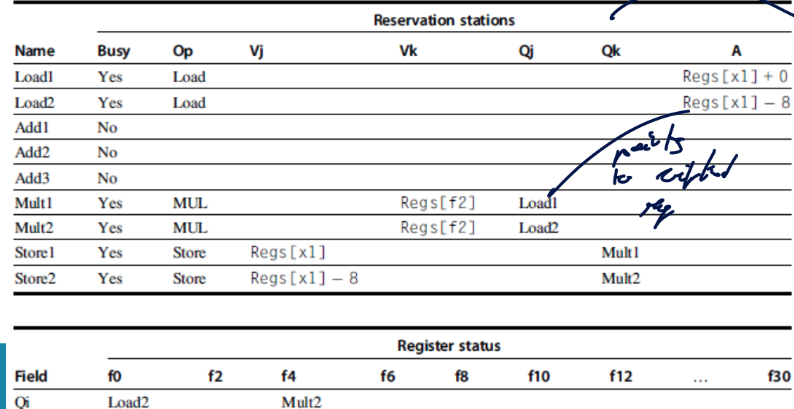
\includegraphics[width=0.75\linewidth]{tomasulo_algo.png}
    \caption{Tomasulo's algorithm}
    \label{fig:tomasulo-label}
\end{figure}

Column names:

\begin{itemize}
    \item \underline{Op:} operation to perform in the unit
    \item \underline{Vj, Vk:} value of source operands, store bufer has result to be stored in Vj field.
    \item \underline{Qj, Qk:} reservation stations producing source registers. If they are = 0 then it means it is ready.
    \item \underline{Busy:} indicates if a reservation station or FU is busy
\end{itemize}

The renaming is \textit{automatically} done inside the reservation stations. We fetch and buffer operands in the reservation station as soon it is available.

At instruction issue, available register file values are copied to reservation stations (eliminate WAR). Specifiers for source operands not available are renamed to the names of the reservation stations when the operand will come from. Values can exist in reservation station or register file. Instructions waiting for input still to be computed, keep track of reservation station which will provide this input.

When we waiting for an operand we keep monitoring the CDB.


\subsubsection{Data bus: Normal vs Common}

In a common data bus we send data to a destination. In a common data bus, we broadcast the results and indicate where it came from. The operation in the reservation stations will listen and write if they see one source matching.

\begin{figure}[H]
    \centering
    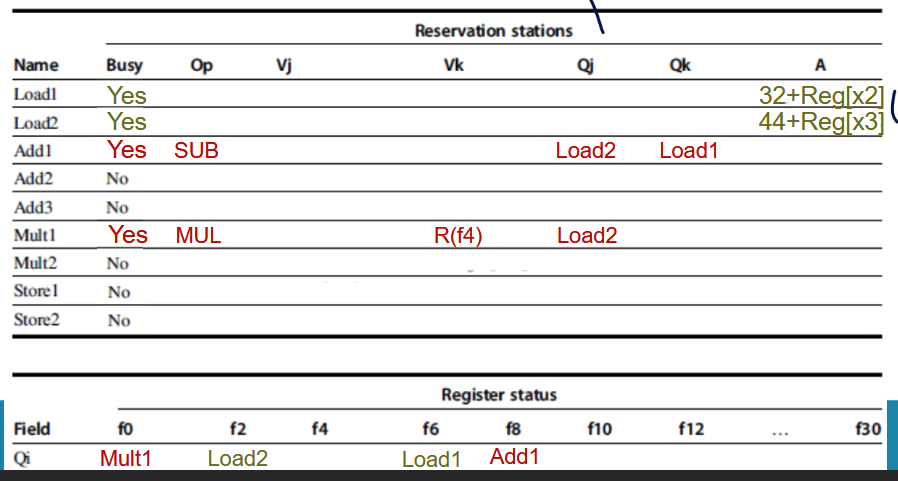
\includegraphics[width=0.45\linewidth]{tomasulo_ex1.png}
    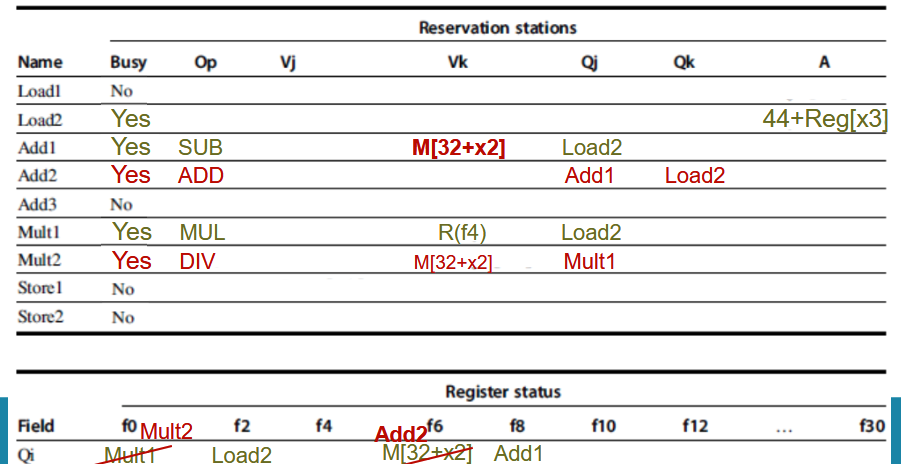
\includegraphics[width=0.45\linewidth]{tomasulo_ex2.png}
    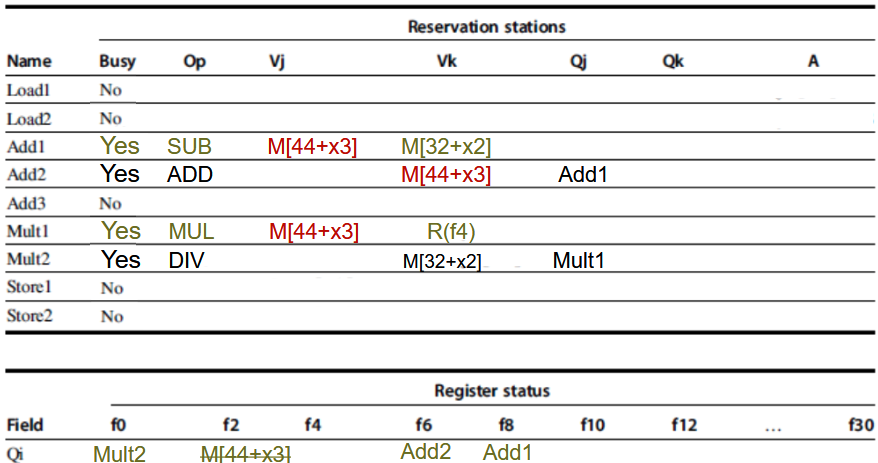
\includegraphics[width=0.45\linewidth]{tomasulo_ex3.png}
    \caption{Tomasulo Example}
    \label{fig:tomasulo-example-label}
\end{figure}

It eliminates the stalls due to WAW and WAR which is pretty beneficial in loops. It also distributes the hazard detection and mitigation logic.

BUT, it requires more hardware and monitoring all tags that pass by on the CDB comes at a cost. We still didn't improve the load store conflict. In fact we could have some \texttt{ld} and \texttt{sd} that could point towards the same address, there is two ways to mitigate this:

\begin{enumerate}
    \item Force load and store to be in order
    \item Check if the \texttt{ld} and \texttt{sd} are allowed to execute:
    \begin{itemize}
        \item \texttt{ld}: only if no uncompleted store with same memory address pending
        \item \texttt{sd}: only if no uncompleted load OR store with the same address pending
    \end{itemize}
\end{enumerate}

Will result in more stalls, we could mitigate it using some ReOrder Buffer. WAW conflicts can result in wrong outcomes !

Also, branch mispredictions and cache misses become very expensive as we need to flush or stall many \textbf{parallel} instructions.

\section{Hardware speculation}

We will try to avoid data dependencies by loading data much in advance. We need to have some speculation since branching causes further throughput losses in Out Of Order processor. That is why we want to do some hardware speculation to guess what instructions should be executed. We increase the basic block size by reshuffling opportunities accross branches. We can however make mistakes.

\subsection{Speculations}

\begin{enumerate}
    \item Speculate that a store: it will not have the same address. Used for store before a load.
    \item Speculate on the outcome of a conditional branch: correct if branch was wrongly predicted but very low miss rates needed.
\end{enumerate}

In speculation and prediction there is 3 big sorts of them:

\begin{enumerate}
    \item Simple: same decision all the time
    \item Static: if the branch is forward we do not take it else we take it. (good for loops and if)
    \item Dynamic: use run-time information
\end{enumerate}

\subsection{Branch Prediction Buffer - BHT}

\begin{figure}[H]
    \centering
    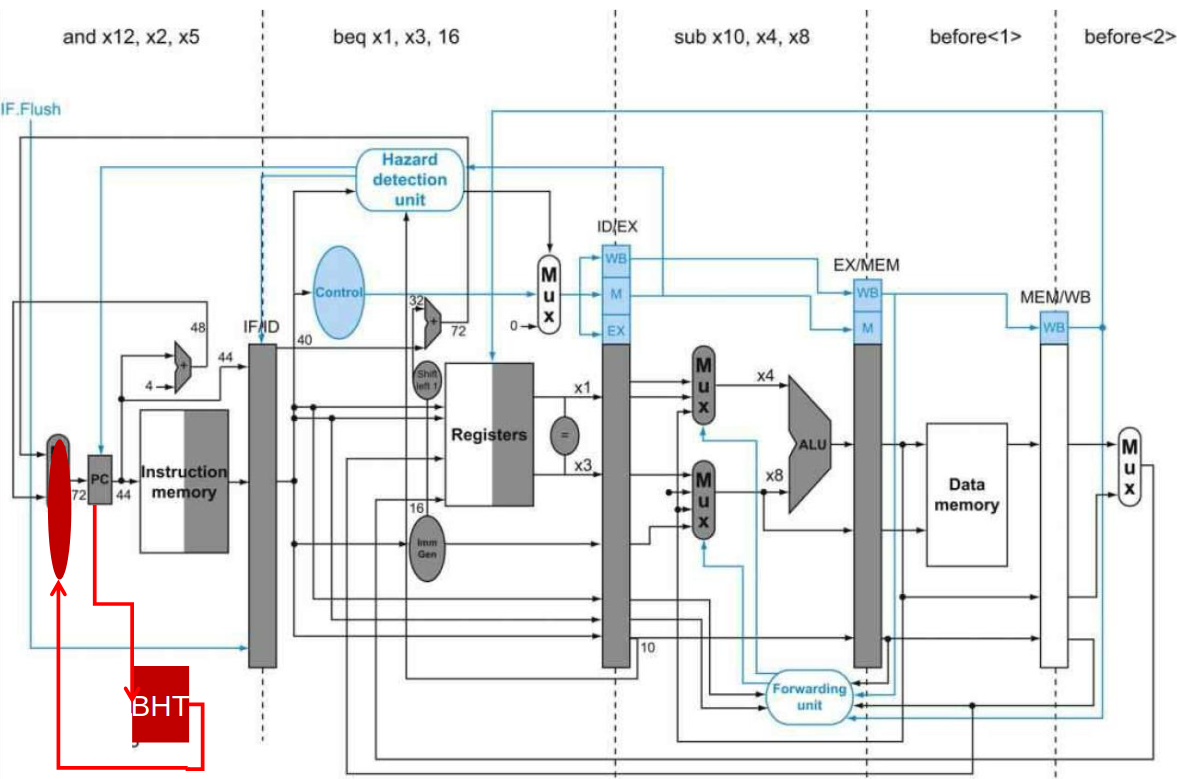
\includegraphics[width=0.65\linewidth]{BHT_hw.png}
    \caption{BHT in Hardware}
    \label{fig:BHT-label}
\end{figure}

We add a little piece of memory in the instructions fetching that stores the \textbf{lower bits of the PC} with the information if the branch was taken or not.

\subsubsection{1-bit prediction buffer}

We simply store one bit indicating if it was taken or not the last time. We need $2^k$ bits for storage space (so it depends on the $k$ lowest bits we want to save). The accuracy is around $85\%$ and for a loop with $N$ iterations we have an accuracy of $\frac{N- 2}{N}$. So it is good for loops with large iterations.

\subsubsection{2-bit prediction buffer}

Here we will store 4 possibles states. We have an extra nuance where we have jump weakly taken and weakly not taken. It is useful for nested loops for example as we will re-enter such loops later and don't want to exit it too soon. It has $2 \cdot 2^k$ bits of storage for a $90\%$ of accuracy. For loops we have a precision of $\frac{N-1}{N}$. Not really effective to add more states.

\subsubsection{Correlating predictors}

Here we exploit informations for m branches and use a sort of \textit{global branch history}. We keep those 2 bit predictors but add the informations about the branches which give us $2 \cdot 2^m \cdot 2^k$ bits storage space. It gives real good results with a $\sim 95\%$ accuracy.

\begin{figure}[H]
    \centering
    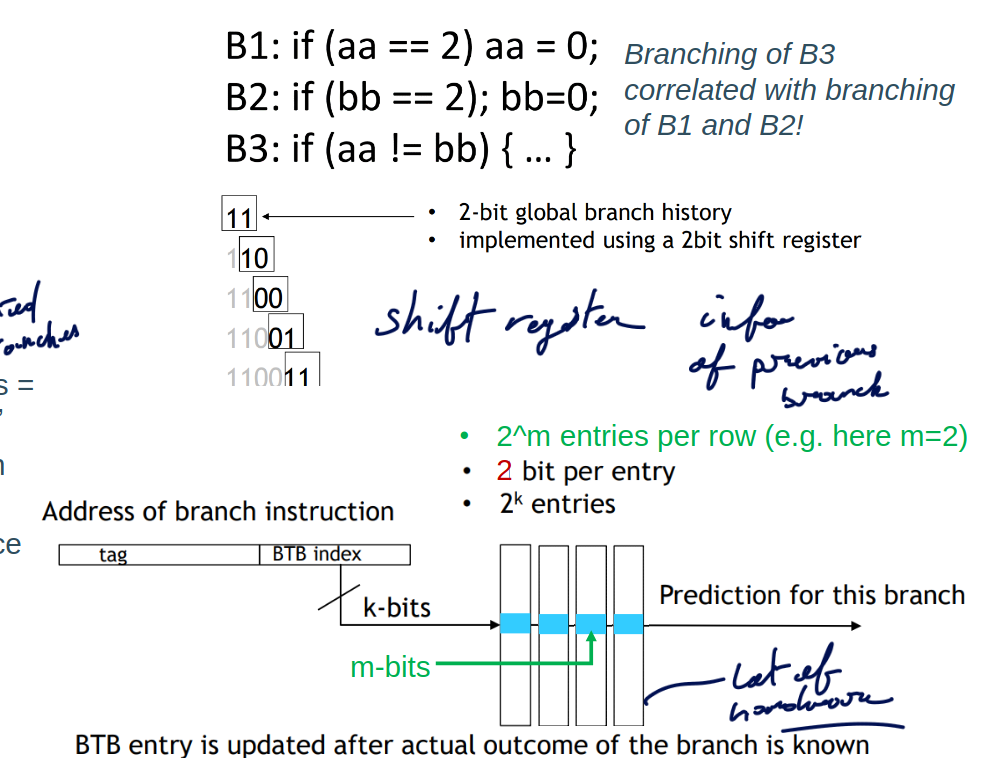
\includegraphics[width=0.5\linewidth]{BHT_m_branch.png}
    \caption{m branch}
    \label{fig:enter-label}
\end{figure}

\subsubsection{g-share}

It is an even more efficient implementation where $m=k$. The idea is to XOR to reduce the storage that is needed. So we will have just around $2 \cdot 2^k$ bits for storage.

\begin{figure}[H]
    \centering
    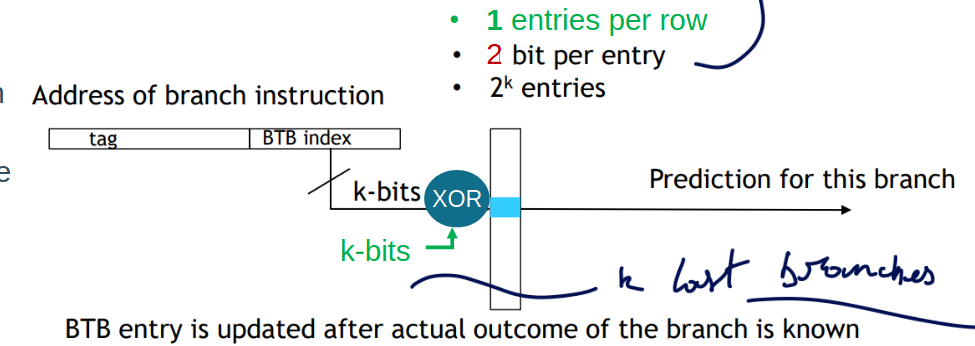
\includegraphics[width=0.5\linewidth]{gshare.png}
    \caption{g-share}
    \label{fig:enter-label}
\end{figure}

\subsubsection{Other techniques}

The best techniques that exists currently reaches $97/98 \%$ of accuracy. It is \textit{tournament predictors, tagged hybrid predictors, ...} using local and global predictors.

\subsection{Branch Target Buffer - BTB}

But in our current implementation, we still loose one or more cycle to compute the branch address so it didn't really help. The BHT tells when or not to take a branch but not where  its taken to !

That's when the BTB comes into play. It is also located in the IF stage and allows to look up the branch target address using the lower PC address bits ! So we use the BHT to trigger a mux and the BTB feeds into this mux.

\begin{figure}[H]
    \centering
    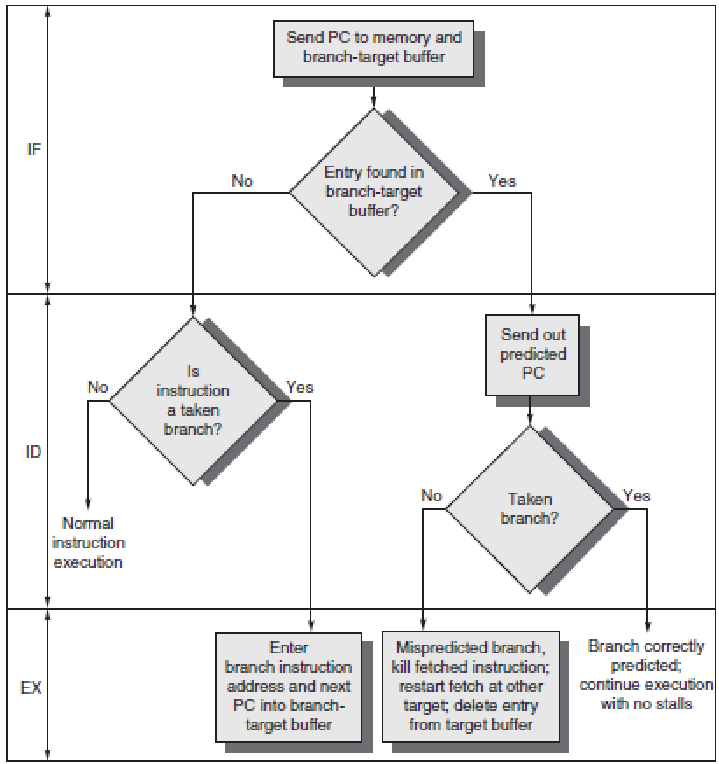
\includegraphics[width=0.5\linewidth]{BTB-BHT.png}
    \caption{BTB and BHT}
    \label{fig:enter-label}
\end{figure}

\subsubsection{Branch Buffer Indexing}

Branch target \& history table do not have to be large. E.g. only 128 entries (k=7) Done every clock cycle:

\begin{itemize}
    \item Index memory with lower k bits of PC
    \item Compare stored PC of memory entry with actual PC
    \item If same, then jump to target address, if not, PC=PC+1
    \item (later): check whether branch did take place; and if needed update BHT, BTB
\end{itemize}

\subsection{Compiler - Hardware speculation}

The compiler can reorder the instructions, move load before branches, ... It is quite crucial in VLIW and in-order processors. It is something that is static.

The hardware can also look ahead for instructions to execute. We put the results of those instructions in a buffer until they are actually correct. We have to flush buffers on incorrect speculation. Superscalar out-of-order, this is something that is dynamic. 

\subsubsection{Danger of Hardware based speculation}

We have to be careful with those transient executions as we should only write back if we are allowed too. We have to add a new piece of hardware that ensures this data integrity.

\section{Out-of-order completion}

It is quite tricky to dynamically schedule a processor. In fact various operations can have various delay due to pipelined operations. So we really have to be extra careful with writing back as the results can come back out of order.

\begin{lstlisting}
    fld  f0, 0(x1)
    fmul f4, f0, f2
    fld  f4, -8(x1)
    ...
\end{lstlisting}

Here, we could already start the second \texttt{fld} operation but we cannot write back to f4 as the multiplication may not have yet finished.

So a good practice is to execute out of order but commit result to registers in order.

\subsection{Reorder Buffer - ROB}

It is a buffer that is designed to hold the result between execution and commit time. It is also able to supply next instructions with \textit{speculative} inputs. Keep an ordered list of the instruction.

Finally, it puts the instruction results back in the original program order after the instructions have finished executions. No more WAW hazards.

We use a round buffer that has different fields:

\begin{enumerate}
    \item \underline{Instruction type:} branch, store, register, ...
    \item \underline{Destination field:} register number or mem address
    \item \underline{Value field:} output value
    \item \underline{Ready field:} completed execution ?
\end{enumerate}

\begin{figure}[H]
    \centering
    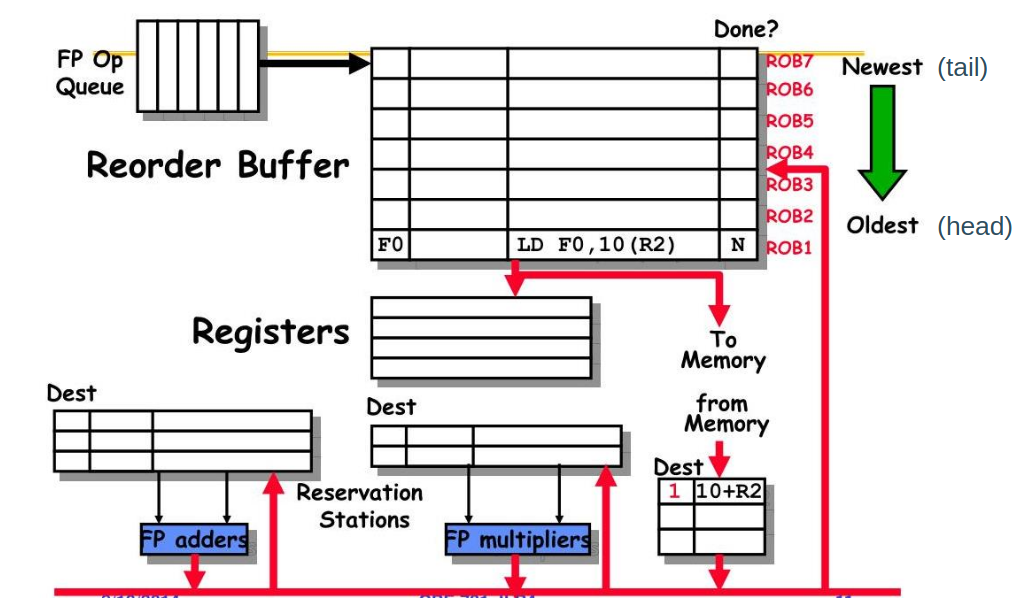
\includegraphics[width=0.7\linewidth]{ROB_reorder.png}
    \caption{Data flow with reorder buffer}
    \label{fig:ROB-reorder-label}
\end{figure}

\subsubsection{Operations with such buffer}

\begin{enumerate}
    \item Issue: allocate RS and ROB, read available operands
    \item Execute: begin execution when operand values are available
    \item Write result: write result and ROB tag on CDB
    \item Commit: when ROB reaches head of ROB, update register. When mispredicted branch reaches head of ROB, discard all entries.
\end{enumerate}

\begin{figure}[H]
    \centering
    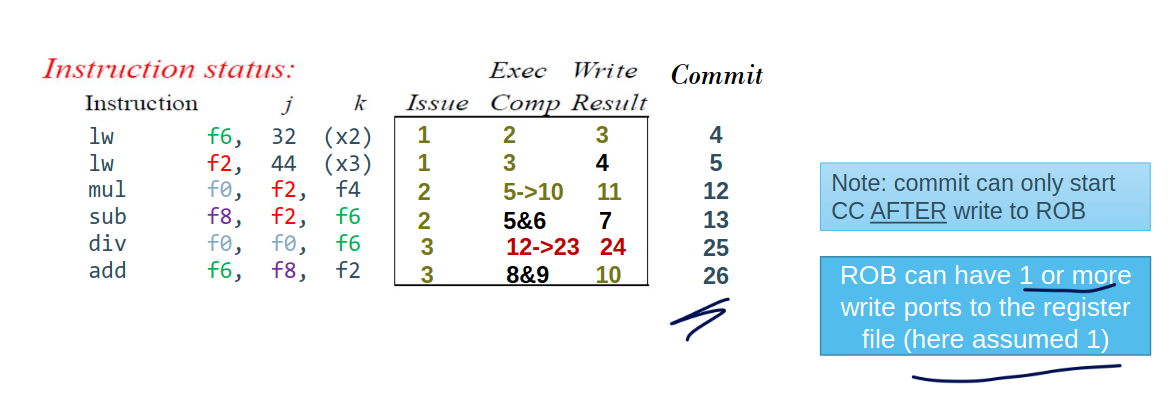
\includegraphics[width=0.75\linewidth]{example_ROB.png}
    \caption{Example of Reorder Buffer}
    \label{fig:enter-label}
\end{figure}

\subsubsection{Commit consequences of speculation}

We start as it was a normal instruction. We then propagate the result up to commit buffer. But before committing, we have to check whether the guess was right. We have to verify if the branch was taken, load store conflict, ... If we messed up we have to roll-back and do the right thing.

We have to keep those results until we determine they are correct.

\begin{figure}[H]
    \centering
    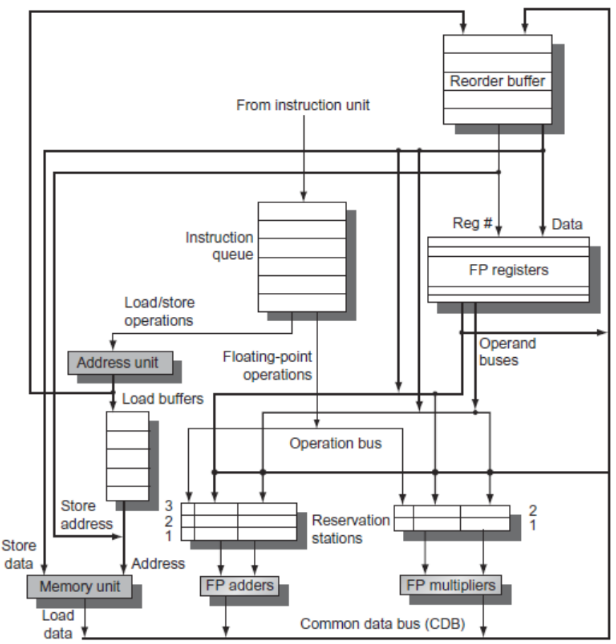
\includegraphics[width=0.5\linewidth]{ROB_architecture.png}
    \caption{ROB architecture - be able to explain it}
    \label{fig:ROB-architecture-label}
\end{figure}

\section{Hybrid forms}

If we want to achieve $CPI<1$ we have to run and complete multiple instructions per clock. To achieve this we have seen 4 main possibilities:

\begin{enumerate}
    \item VLIW where it is statically scheduled
    \item In-order superscalar processors (static and dynamic scheduling)
    \item Dynamically scheduled OOO superscalar processors, single thread
    \item Dynamically scheduled OOO superscalar processors, multithreading 
\end{enumerate}

\begin{figure}[H]
    \centering
    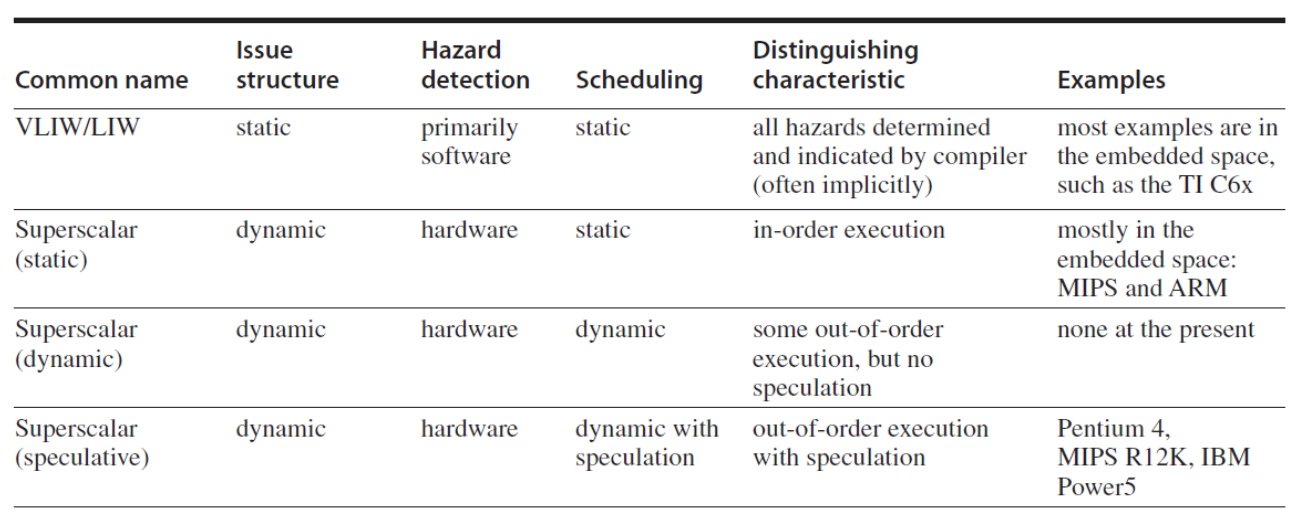
\includegraphics[width=0.8\linewidth]{summary_multiple_issue.png}
    \caption{Summary multiple-issue}
    \label{fig:enter-label}
\end{figure}

If we look at the roofline diagram, we can see how dynamic scheduling and multiple issue processor enables to reach new limits in what is possible on a processor.

\chapter{Exploiting Data Level Parllelism (DLP)}
\chapter{Exploiting Thread Level Parallelism (TLP)}
\chapter{Zooming out: Trends and system level considerations}




\end{document}
